\chapter{Random Variables}

%% Introduction %%%%%%%%%%%%%%%%%%%%%%%%%%%%%%%%%%%%%%%%%%%%%%%%%%%%%%%%%%%%%%%
So far we focused on probabilities of \term{events} ---that you win the
Monty Hall game; that you have a rare medical condition, given that you
tested positive; \dots.  Now we focus on quantitative questions: \emph{How
  many} contestants must play the Monty Hall game until one of them
finally wins? \dots {\em How long} will this condition last?  {\em How
  much} will I lose playing 6.042 games all day?  \emph{Random variables}
are the mathematical tool for addressing such questions.


%% Random Variables %%%%%%%%%%%%%%%%%%%%%%%%%%%%%%%%%%%%%%%%%%%%%%%%%%%%%%%%%%%
\hyperdef{random}{vars}{\section{Random Variables}}

\begin{definition}
  A random variable, $R$, on a probability space is a function whose
  domain is the sample space.
\end{definition}
The codomain of $R$ can be anything, but will usually be a subset of the
real numbers.  Notice that the name ``random variable'' is a misnomer;
random variables are actually functions!

\subsection{Counting Coin Flips}
Consider the experiment of tossing three independent, unbiased coins.  Let
$C$ be the number of heads that appear.  Let $M = 1$ if the three coins
come up all heads or all tails, and let $M = 0$ otherwise.  Now every
outcome of the three coin flips uniquely determines the values of $C$ and
$M$.  For example, if we flip heads, tails, heads, then $C = 2$ and $M =
0$.  If we flip tails, tails, tails, then $C = 0$ and $M = 1$.  In effect,
$C$ counts the number of heads, and $M$ indicates whether all the coins
match.

Since each outcome uniquely determines $C$ and $M$, we can regard them
as functions mapping outcomes to numbers.  For this experiment, the
sample space is:
\begin{eqnarray*}
\sspace & = & \set{ HHH, HHT, HTH, HTT, THH, THT, TTH, TTT }.
\end{eqnarray*}
Now $C$ is a function that maps each outcome in the sample space to a 
number as follows:
\[
\begin{array}{rclcrcl}
C(HHH) & = & 3 & \quad & C(THH) & = & 2 \\
C(HHT) & = & 2 & \quad & C(THT) & = & 1 \\
C(HTH) & = & 2 & \quad & C(TTH) & = & 1 \\
C(HTT) & = & 1 & \quad & C(TTT) & = & 0.
\end{array}
\]
Similarly, $M$ is a function mapping each outcome another way:
\[
\begin{array}{rclcrcl}
M(HHH) & = & 1 & \quad & M(THH) & = & 0 \\
M(HHT) & = & 0 & \quad & M(THT) & = & 0 \\
M(HTH) & = & 0 & \quad & M(TTH) & = & 0 \\
M(HTT) & = & 0 & \quad & M(TTT) & = & 1.
\end{array}
\]
So $C$ and $M$ are \term{random variables}.

\subsection{Indicator Random Variables}

An \term{indicator random variable} (or simply an \term{indicator}, or
a \term{Bernoulli random variable}) is a random variable that maps
every outcome to either 0 or 1.  The random variable $M$ is an
example.  If all three coins match, then $M=1$; otherwise, $M = 0$.

Indicator random variables are closely related to events.  In
particular, an indicator partitions the sample space into those
outcomes mapped to 1 and those outcomes mapped to 0.  For example, the
indicator $M$ partitions the sample space into two blocks as follows:
\[
\underbrace{HHH \quad TTT}_{\text{$M = 1$}} \quad
\underbrace{HHT \quad HTH \quad HTT \quad
        THH \quad THT \quad TTH}_{\text{$M = 0$}}.
\]

In the same way, an event, $E$, partitions the sample space into those
outcomes in $E$ and those not in $E$.  So $E$ is naturally associated with
an indicator random variable, $I_E$, for the event, where $I_E(p) = 1$ for
outcomes $p \in E$ and $I_E(p) = 0$ for outcomes $p \notin E$.  Thus,
$M=I_F$ where $F$ is the event that all three coins match.

\subsection{Random Variables and Events}

There is a strong relationship between events and more general random
variables as well.  A random variable that takes on several values
partitions the sample space into several blocks.  For example, $C$
partitions the sample space as follows:
\[
\underbrace{TTT}_{\text{$C = 0$}} \quad
\underbrace{TTH \quad THT \quad HTT}_{\text{$C = 1$}} \quad
\underbrace{THH \quad HTH \quad HHT}_{\text{$C = 2$}} \quad
\underbrace{HHH}_{\text{$C = 3$}}.
\]
Each block is a subset of the sample space and is therefore
an event.  Thus, we can regard an equation or inequality involving a
random variable as an event.  For example, the event that $C = 2$
consists of the outcomes $THH$, $HTH$, and $HHT$.  The event $C \leq
1$ consists of the outcomes $TTT$, $TTH$, $THT$, and $HTT$.

Naturally enough, we can talk about the probability of events defined
by properties of random variables.  For example, 
\begin{eqnarray*}
\pr{C = 2}
        & = &   \pr{THH} + \pr{HTH} + \pr{HHT} \\
        & = &   \frac{1}{8} + \frac{1}{8} + \frac{1}{8} =  \frac{3}{8}.
\end{eqnarray*}

\iffalse

As another example:
\begin{eqnarray*}
\pr{M = 1}
        & = &   \pr{TTT} + \pr{HHH}\\
        & = &   \frac{1}{8} + \frac{1}{8} =    \frac{1}{4}.
\end{eqnarray*}



\subsection{Conditional Probability}

Mixing conditional probabilities and events involving random variables
creates no new difficulties.  For example, $\prcond{C \geq 2}{M = 0}$
is the probability that at least two coins are heads ($C \geq 2$),
given that not all three coins are the same ($M = 0$).  We can compute
this probability using the definition of conditional probability:
\begin{eqnarray*}
\prcond{C \geq 2}{M = 0}
        & = &   \frac{\pr{[C \geq 2] \intersect [M = 0]}}{\pr{M = 0}} \\
        & = &   \frac{\pr{\set{THH, HTH, HHT}}}
                        {\pr{\set{THH, HTH, HHT, HTT, THT, TTH }}} \\
        & = &   \frac{3/8}{6/8} = \frac{1}{2}.
\end{eqnarray*}
The expression $[C \geq 2] \intersect [M = 0]$ on the first line may look odd;
what is the set operation $\intersect$ doing between an inequality and an
equality?  But recall that, in this context, $[C \geq 2]$ and $[M = 0]$
are \emph{events}, namely, \emph{sets} of outcomes.
\fi

\subsection{Independence}

The notion of independence carries over from events to random
variables as well.  Random variables $R_1$ and $R_2$ are
\term{independent} iff for all $x_1$ in the codomain
of $R_1$, and $x_2$  in the codomain of $R_2$, we have:
\[
\pr{R_1 = x_1 \QAND R_2 = x_2}  =  \pr{R_1 = x_1} \cdot \pr{R_2 = x_2}.
\]
As with events, we can formulate independence for random
variables in an equivalent and perhaps more intuitive way: random
variables $R_1$ and $R_2$ are independent if for all $x_1$ and $x_2$
\[
\prcond{R_1 = x_1}{R_2 = x_2}  =  \pr{R_1 = x_1}.
\]
whenever the lefthand conditional probability is defined, that is,
whenever $\pr{R_2 = x_2} > 0$.

As an example, are $C$ and $M$ independent?  Intuitively, the answer
should be ``no''.  The number of heads, $C$, completely determines
whether all three coins match; that is, whether $M = 1$.  But, to
verify this intuition, we must find some $x_1, x_2 \in \reals$
such that:
\[
\pr{C = x_1 \QAND M = x_2} \neq \pr{C = x_1} \cdot \pr{M = x_2}.
\]
One appropriate choice of values is $x_1 = 2$ and $x_2 = 1$.
In this case, we have:
\[
\pr{C = 2 \QAND M = 1} = 0 \neq \dfrac{1}{4} \cdot \dfrac{3}{8} = \pr{M
= 1} \cdot \pr{C = 2}.
\]
The first probability is zero because we never have exactly two heads ($C
= 2$) when all three coins match ($M = 1$).  The other two probabilities
were computed earlier.

On the other hand, let $H_1$ be the indicator variable for event that the
first flip is a Head, so
\[
[H_1 = 1] = \set{HHH, HTH, HHT, HTT}.
\]
Then $H_1$ is independent of $M$, since
\begin{align*}
\pr{M=1} & = 1/4 = \prcond{M=1}{H_1=1} = \prcond{M=1}{H_1=0}\\
\pr{M=0} & = 3/4 = \prcond{M=0}{H_1=1} = \prcond{M=0}{H_1=0}
\end{align*}
This example is an instance of a simple
\begin{lemma}
  Two events are independent iff their indicator variables are
  independent.
\end{lemma}
As with events, the notion of independence generalizes to more than two
random variables.
\begin{definition}
Random variables $R_1, R_2, \dots, R_n$ are \term{mutually independent} iff
\begin{eqnarray*}
\lefteqn{\pr{R_1 = x_1 \QAND R_2 = x_2 \QAND \cdots \QAND R_n = x_n}}\\
        & = & \pr{R_1 = x_1} \cdot \pr{R_2 = x_2} \cdots \pr{R_n = x_n}.
\end{eqnarray*}
for all $x_1, x_2, \dots, x_n$.
\end{definition}

It is a simple exercise to show that the probability that any {\em
subset} of the variables takes a particular set of values is equal to the
product of the probabilities that the individual variables take their
values.  Thus, for example, if $R_1, R_2, \dots, R_{100}$ are mutually
independent random variables, then it follows that:
\[
\pr{R_1 = 7 \QAND R_7 = 9.1 \QAND R_{23} = \pi} = \pr{R_1 = 7} \cdot
\pr{R_7 = 9.1} \cdot \pr{R_{23} = \pi}.
\]

%% Random Variables Problems %%%%%%%%%%%%%%%%%%%%%%%%%%%%%%%%%%%%%%%%%%%%%%%%%%
%\startclassproblems
%\pinput{CP_}


%% The Birthday Principle %%%%%%%%%%%%%%%%%%%%%%%%%%%%%%%%%%%%%%%%%%%%%%%%%%%%%
\section{The Birthday Principle}

There are 100 students in a lecture hall.  What is the probability that
some two people share a birthday?  Maybe about $1/3$?  Let's check!  We'll
use the following two variables throughout our analysis:

\begin{itemize}

\item Let $n$ be the number of people in the group.

\item Let $d$ be the number of days in the year.

\item Let $D$ be the number of pairs of students with the same birthday.

\end{itemize}

We'll assume that a random choice of a student is made independently of
the any other choices of students.  For simplicity, we'll assume that the
probability that a randomly chosen student has a given birthday is 1/365.
This assumption is not really true, since more babies are born at certain
times of year.  However, our analysis of this problem applies to many
situations in Computer Science that are unaffected by leap days, snow days
or Spring fever, so we won't dwell on those complications.

A sensible sample space to model this experiment consists of all ways of
assigning birthdays to the people of the group.  There are $d^n$ such
assignments, since the first person can have $d$ different birthdays, the
second person can have $d$ different birthdays, and so forth.
Furthermore, every such assignment is equally probable by our assumption
that birthdays are equally likely and independent of each other.

Now the event that some two students have the same birthday can be
expressed as $[D>0]$.  It turns out to be be easier to calculate the
complement event $[D=0]$ that everyone has a distinct birthday, which is
good enough since $\pr{D>0} = 1 - \pr{D=0}$.

Anyway, the event $[D=0]$ consists of $d (d - 1) (d - 2) \cdots (d - n +
1)$ outcomes, since we can select the birthday of the first person in $d$
days, the birthday of the second person in $d - 1$ ways, and so forth.
Therefore, the probability that everyone has a different birthday is:
\begin{align*}
\pr{D=0} & = \frac{d (d - 1) (d - 2) \cdots (d - n + 1)}{d^n}.
\end{align*}
For $n=100$, this probability is actually fantastically small ---less
than one in a million!  If there are 100 people in a room, two are
almost certain to share a birthday.

Let's rewrite the right side of the preceding equation in a more
insightful form that allows us to use the fact that $e^x >1+x$ for all
$x$.\footnote{This approximation is obtained by truncating the Taylor
series $e^{-x} = 1 - x + x^2/2! - x^3/3! + \cdots$.  The approximation
$e^{-x} \approx 1 - x$ is pretty accurate when $x$ is small.}
\begin{align*}
\pr{D=0} & = \left(1 - \frac{0}{d}\right)
           \left(1 - \frac{1}{d}\right)
           \left(1 - \frac{2}{d}\right) 
           \cdots
           \left(1 - \frac{n - 1}{d}\right)\\
       & < e^0 \cdot e^{-1/d} \cdot e^{-2/d} \cdots e^{-(n-1)/d} \\
       & = e^{-\frac{\sum_{i=1}^{n-1} i}{d}}\\
       & = e^{\dfrac{-n(n-1)}{2d}} = e^{-\dfrac{\binom{n}{2}}{d}}.
\end{align*}

The exponent $\binom{n}{2}/d$ in the final expression above is close to
$1$ when $n \approx \sqrt{2d}$.  In this case, the probability that two
people share a birthday is close to $1/e$ which is roughly the break-even
point, where it's equally likely whether or not a couple of people will
share a birthday.  This leads to a rule called the \term{Birthday
Principle}, which is useful in many contexts in Computer Science:
\begin{quote}
If there are $d$ days in a year and $\sqrt{2d}$ people in a
room, then the probability that two share a birthday is about 
$1 - 1/e \approx 0.632$.
\end{quote}
For example, this principle says that if you have $\sqrt{2 \cdot 365}
\approx 27$ people in a room, then the probability that two share a
birthday is about $0.632$.  The actual probability is about $0.626$,
so the approximation is quite good.

The Birthday Principle is a great rule of thumb with surprisingly many
applications.  For example, cryptographic systems and digital signature
schemes must be hardened against ``birthday attacks''.  The principle also
tells us how many items can be inserted into a hash table before one
starts to experience collisions.

%% The Birthday Principle Problems %%%%%%%%%%%%%%%%%%%%%%%%%%%%%%%%%%%%%%%%%%%%
%\startclassproblems
%\pinput{CP_}


%% Probability Distributions %%%%%%%%%%%%%%%%%%%%%%%%%%%%%%%%%%%%%%%%%%%%%%%%%%
\section{Probability Distributions}

A random variable is function whose domain is the sample space of an
experiment, but random variables with that show up in completely different
experiments wind up behaving in much the same way because they have the
same probabilities of taking different values.  Namely, random variables
on different probability spaces may wind up having the same probability
density function.

\begin{definition}
Let $R$ be a random variable with with codomain $V$.
The \term{probability density function (pdf)} of $R$
is a function $\pdf_R : V \to [0,1]$ defined by:
%
\[
\pdf_R(x) \eqdef \begin{cases}
            \pr{R = x} & \text{if } x \in \range{R},\\
             0 & \text{if } x \notin \range{R}.
           \end{cases}
\]
\end{definition}
%
A consequence of this definition is that
%
\[
\sum_{x \in \range{R}} \pdf_R(x) = 1.
\]
This follows because $R$ has a value for each outcome, so summing the
probabilities over all outcomes is the same as summing over the
probabilities of each value in the range of $R$.

As an example, let's return to the experiment of rolling two fair,
independent dice.  As before, let $T$ be the total of the two rolls.
This random variable takes on values in the set $V = \set{2, 3,
\dots, 12}$.  A plot of the probability density function is shown
below:
%
\begin{center}
\begin{picture}(305,110)(-75,-40)
%\put(-75,-40){\dashbox(305,110)} % bounding box
\put(0,0){\vector(1,0){230}}
\put(0,0){\vector(0,1){70}}
\put(-1,60){\line(1,0){2}}
\put(-15,60){\makebox(0,0){{\small $6/36$}}}
\put(-1,30){\line(1,0){2}}
\put(-15,30){\makebox(0,0){{\small $3/36$}}}
\put(-50,40){\makebox(0,0){$\pdf_R(x)$}}
\put(120,-30){\makebox(0,0){$x \in V$}}
\put(0,0){\framebox(20,10){}}
\put(10,-10){\makebox(0,0){2}}
\put(20,0){\framebox(20,20){}}
\put(30,-10){\makebox(0,0){3}}
\put(40,0){\framebox(20,30){}}
\put(50,-10){\makebox(0,0){4}}
\put(60,0){\framebox(20,40){}}
\put(70,-10){\makebox(0,0){5}}
\put(80,0){\framebox(20,50){}}
\put(90,-10){\makebox(0,0){6}}
\put(100,0){\framebox(20,60){}}
\put(110,-10){\makebox(0,0){7}}
\put(120,0){\framebox(20,50){}}
\put(130,-10){\makebox(0,0){8}}
\put(140,0){\framebox(20,40){}}
\put(150,-10){\makebox(0,0){9}}
\put(160,0){\framebox(20,30){}}
\put(170,-10){\makebox(0,0){10}}
\put(180,0){\framebox(20,20){}}
\put(190,-10){\makebox(0,0){11}}
\put(200,0){\framebox(20,10){}}
\put(210,-10){\makebox(0,0){12}}
\end{picture}
\end{center}
%
The lump in the middle indicates that sums close to 7 are the most
likely.  The total area of all the rectangles is 1 since the dice must
take on exactly one of the sums in $V = \set{2, 3, \dots, 12}$.

A closely-related idea is the \term{cumulative distribution function
(cdf)} for a random variable $R$ whose codomain is real numbers.  This is a
function $\cdf_R : \reals \to [0,1]$ defined by:
%
\[
\cdf_R(x) = \pr{R \leq x}
\]
%
As an example, the cumulative distribution function for the random
variable $T$ is shown below:
%
\begin{center}
\begin{picture}(305,155)(-75,-40)
%\put(-75,-40){\dashbox(305,155)} % bounding box
\put(0,0){\vector(1,0){230}}
\put(0,0){\vector(0,1){115}}
\put(-1,108){\line(1,0){2}}
\put(-15,108){\makebox(0,0){{\small $1$}}}
\put(-1,54){\line(1,0){2}}
\put(-15,54){\makebox(0,0){{\small $1/2$}}}
\put(-15,0){\makebox(0,0){{\small $0$}}}
\put(-50,81){\makebox(0,0){$\cdf_R(x)$}}
\put(120,-30){\makebox(0,0){$x \in V$}}
\put(0,0){\framebox(20,3){}}
\put(10,-10){\makebox(0,0){2}}
\put(20,0){\framebox(20,9){}}
\put(30,-10){\makebox(0,0){3}}
\put(40,0){\framebox(20,18){}}
\put(50,-10){\makebox(0,0){4}}
\put(60,0){\framebox(20,30){}}
\put(70,-10){\makebox(0,0){5}}
\put(80,0){\framebox(20,45){}}
\put(90,-10){\makebox(0,0){6}}
\put(100,0){\framebox(20,63){}}
\put(110,-10){\makebox(0,0){7}}
\put(120,0){\framebox(20,78){}}
\put(130,-10){\makebox(0,0){8}}
\put(140,0){\framebox(20,90){}}
\put(150,-10){\makebox(0,0){9}}
\put(160,0){\framebox(20,99){}}
\put(170,-10){\makebox(0,0){10}}
\put(180,0){\framebox(20,105){}}
\put(190,-10){\makebox(0,0){11}}
\put(200,0){\framebox(20,108){}}
\put(210,-10){\makebox(0,0){12}}
\end{picture}
\end{center}
%
The height of the $i$-th bar in the cumulative distribution function
is equal to the \textit{sum} of the heights of the leftmost $i$ bars
in the probability density function.  This follows from the
definitions of pdf and cdf:
%
\begin{align*}
\cdf_R(x) & = \pr{R \leq x} \\
          & = \sum_{y \leq x} \pr{R = y} \\
          & = \sum_{y \leq x} \pdf_R(y)
\end{align*}

In summary, $\pdf_R(x)$ measures the probability that $R = x$ and
$\cdf_R(x)$ measures the probability that $R \leq x$.  Both the
$\pdf_R$ and $\cdf_R$ capture the same information about the random
variable $R$--- you can derive one from the other ---but sometimes one
is more convenient.  The key point here is that neither the
probability density function nor the cumulative distribution function
involves the sample space of an experiment.

\iffalse
Thus, through these
functions, we can study random variables without reference to a
particular experiment.
\fi


We'll now look at three important distributions and some applications.

\subsection{Bernoulli Distribution}

Indicator random variables are perhaps the most common type because of
their close association with events.  The probability density function
of an indicator random variable $B$ is always
%
\begin{align*}
\pdf_B(0) & = p \\
\pdf_B(1) & = 1 - p \\
\end{align*}
%
where $0 \leq p \leq 1$.  The corresponding cumulative distribution
function is:
%
\begin{align*}
\cdf_B(0) & = p \\
\cdf_B(1) & = 1
\end{align*}
%
%This is called the \term{Bernoulli distribution}. 
%The number of heads
%flipped on a (possibly biased) coin has a Bernoulli distribution.

\subsection{Uniform Distribution}

A random variable that takes on each possible value with the same
probability is called \term{uniform}.  For example, the probability
density function of a random variable $U$ that is uniform on the set
$\set{1, 2, \dots, N}$ is:
%
\begin{align*}
\pdf_U(k) = \frac{1}{N}
\end{align*}
%
And the cumulative distribution function is:
%
\begin{align*}
\cdf_U(k) = \frac{k}{N}
\end{align*}
%
Uniform distributions come up all the time.  For example, the number
rolled on a fair die is uniform on the set $\set{1, 2, \dots, 6}$.

\iffalse

\subsection{The Numbers Game}

Let's play a game!  I have two envelopes.  Each contains an integer in
the range $0, 1, \dots, 100$, and the numbers are distinct.  To win
the game, you must determine which envelope contains the larger
number.  To give you a fighting chance, I'll let you peek at the
number in one envelope selected at random.  Can you devise a strategy
that gives you a better than 50\% chance of winning?

For example, you could just pick an evelope at random and guess that
it contains the larger number.  But this strategy wins only 50\% of
the time.  Your challenge is to do better.

So you might try to be more clever.  Suppose you peek in the left
envelope and see the number 12.  Since 12 is a small number, you might
guess that that other number is larger.  But perhaps I'm sort of
tricky and put small numbers in \textit{both} envelopes.  Then your
guess might not be so good!

An important point here is that the numbers in the envelopes may
\textit{not} be random.  I'm picking the numbers and I'm choosing them
in a way that I think will defeat your guessing strategy.  I'll only
use randomization to choose the numbers if that serves \textit{my}
end:  making you lose!

\subsubsection{Intuition Behind the Winning Strategy}

Amazingly, there is a strategy that wins more than 50\% of the time,
regardless of what numbers I put in the envelopes!

Suppose that you somehow knew a number $x$ \textit{between} my lower
number and higher numbers.  Now you peek in an envelope and see one or
the other.  If it is bigger than $x$, then you know you're peeking at
the higher number.  If it is smaller than $x$, then you're peeking at
the lower number.  In other words, if you know a number $x$ between
my lower and higher numbers, then you are certain to win the game.

The only flaw with this brilliant strategy is that you do \textit{not}
know $x$.  Oh well.

But what if you try to \textit{guess} $x$?  There is some probability
that you guess correctly.  In this case, you win 100\% of the time.
On the other hand, if you guess incorrectly, then you're no worse off
than before; your chance of winning is still 50\%.  Combining these
two cases, your overall chance of winning is better than 50\%!

Informal arguments about probability, like this one, often sound
plausible, but do not hold up under close scrutiny.  In contrast, this
argument sounds completely implausible--- but is actually correct!

\subsubsection{Analysis of the Winning Strategy}

For generality, suppose that I can choose numbers from the set
$\set{0, 1, \dots, n}$.  Call the lower number $L$ and the higher
number $H$.

Your goal is to guess a number $x$ between $L$ and $H$.  To avoid
confusing equality cases, you select $x$ at random from among the
half-integers:
%
\[
\set{\frac{1}{2},\ 1\frac{1}{2},\ 2\frac{1}{2},\ \dots,\ n - \frac{1}{2}}
\]
%
But what probability distribution should you use?

The uniform distribution turns out to be your best bet.  An informal
justification is that if I figured out that you were unlikely to pick
some number--- say $50\frac{1}{2}$--- then I'd always put 50 and 51 in
the evelopes.  Then you'd be unlikely to pick an $x$ between $L$ and
$H$ and would have less chance of winning.

After you've selected the number $x$, you peek into an envelope and
see some number $p$.  If $p > x$, then you guess that you're looking
at the larger number.  If $p < x$, then you guess that the other
number is larger.

All that remains is to determine the probability that this strategy
succeeds.  We can do this with the usual four step method and a tree
diagram.

\noindent \textbf{Step 1: Find the sample space. }  You either choose
$x$ too low ($< L$), too high ($> H$), or just right ($L < x < H$).
Then you either peek at the lower number ($p = L$) or the higher
number ($p = H$).  This gives a total of six possible outcomes.
%
\begin{center}
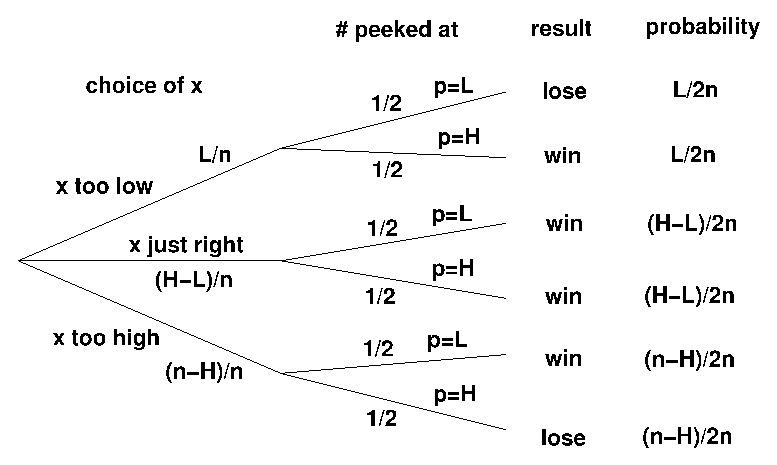
\includegraphics[height=2.5in]{figures/numbers-game}
\end{center}

\noindent \textbf{Step 2: Define events of interest. } The four
outcomes in the event that you win are marked in the tree diagram.

\noindent \textbf{Step 3: Assign outcome probabilities. } First, we
assign edge probabilities.  Your guess $x$ is too low with probability
$L/n$, too high with probability $(n-H)/n$, and just right with
probability $(H-L)/n$.  Next, you peek at either the lower or higher
number with equal probability.  Multiplying along root-to-leaf paths
gives the outcome probabilities.

\noindent \textbf{Step 4: Compute event probabilities. }  The
probability of the event that you win is the sum of the probabilities
of the four outcomes in that event:
%
\begin{align*}
\pr{\text{win}}
    & = \frac{L}{2n} + \frac{H-L}{2n} + \frac{H-L}{2n}  + \frac{n-H}{2n} \\
    & = \frac{1}{2} + \frac{H-L}{2n} \\
    & \geq \frac{1}{2} + \frac{1}{2n}
\end{align*}
%
The final inequality relies on the fact that the higher number $H$ is
at least 1 greater than the lower number $L$ since they are required
to be distinct.

Sure enough, you win with this strategy more than half the time,
regardless of the numbers in the envelopes!  For example, if I choose
numbers in the range $0, 1, \dots, 100$, then you win with probability at
least $\frac{1}{2} + \frac{1}{200} = 50.5\%$.  Even better, if I'm allowed
only numbers in the range $0, \dots, 10$, then your probability of
winning rises to 55\%!  By Las Vegas standards, those are great odds!
\fi

\subsection{Binomial Distribution}

Of the more complex distributions, the \term{binomial distribution} is
surely the most important in Computer Science.  The standard example
of a random variable with a binomial distribution is the number of
heads that come up in $n$ independent flips of a coin; call this
random variable $H_n$.  If the coin is fair, then $H_n$ has an
\textit{unbiased binomial density function}:
%
\[
\pdf_{H_n}(k) = \binom{n}{k} 2^{-n}.
\]
%
This follows because there are $\binom{n}{k}$ sequences of $n$ coin
tosses with exactly $k$ heads, and each such sequence has probability
$2^{-n}$.

Here is a plot of the unbiased probability density function
$\pdf_{H_n}(k)$ corresponding to $n = 20$ coins flips.  The most likely
outcome is $k = 10$ heads, and the probability falls off rapidly for
larger and smaller values of $k$.  These falloff regions to the left and
right of the main hump are usually called the \term{tails of the
distribution}.
%
\begin{center}
% GNUPLOT: LaTeX picture
\setlength{\unitlength}{0.240900pt}
\ifx\plotpoint\undefined\newsavebox{\plotpoint}\fi
\sbox{\plotpoint}{\rule[-0.200pt]{0.400pt}{0.400pt}}%
\begin{picture}(1500,900)(0,0)
\font\gnuplot=cmr10 at 10pt
\gnuplot
\sbox{\plotpoint}{\rule[-0.200pt]{0.400pt}{0.400pt}}%
\put(140.0,82.0){\rule[-0.200pt]{4.818pt}{0.400pt}}
\put(120,82){\makebox(0,0)[r]{0}}
\put(1419.0,82.0){\rule[-0.200pt]{4.818pt}{0.400pt}}
\put(140.0,168.0){\rule[-0.200pt]{4.818pt}{0.400pt}}
\put(120,168){\makebox(0,0)[r]{0.02}}
\put(1419.0,168.0){\rule[-0.200pt]{4.818pt}{0.400pt}}
\put(140.0,255.0){\rule[-0.200pt]{4.818pt}{0.400pt}}
\put(120,255){\makebox(0,0)[r]{0.04}}
\put(1419.0,255.0){\rule[-0.200pt]{4.818pt}{0.400pt}}
\put(140.0,341.0){\rule[-0.200pt]{4.818pt}{0.400pt}}
\put(120,341){\makebox(0,0)[r]{0.06}}
\put(1419.0,341.0){\rule[-0.200pt]{4.818pt}{0.400pt}}
\put(140.0,428.0){\rule[-0.200pt]{4.818pt}{0.400pt}}
\put(120,428){\makebox(0,0)[r]{0.08}}
\put(1419.0,428.0){\rule[-0.200pt]{4.818pt}{0.400pt}}
\put(140.0,514.0){\rule[-0.200pt]{4.818pt}{0.400pt}}
\put(120,514){\makebox(0,0)[r]{0.1}}
\put(1419.0,514.0){\rule[-0.200pt]{4.818pt}{0.400pt}}
\put(140.0,601.0){\rule[-0.200pt]{4.818pt}{0.400pt}}
\put(120,601){\makebox(0,0)[r]{0.12}}
\put(1419.0,601.0){\rule[-0.200pt]{4.818pt}{0.400pt}}
\put(140.0,687.0){\rule[-0.200pt]{4.818pt}{0.400pt}}
\put(120,687){\makebox(0,0)[r]{0.14}}
\put(1419.0,687.0){\rule[-0.200pt]{4.818pt}{0.400pt}}
\put(140.0,774.0){\rule[-0.200pt]{4.818pt}{0.400pt}}
\put(120,774){\makebox(0,0)[r]{0.16}}
\put(1419.0,774.0){\rule[-0.200pt]{4.818pt}{0.400pt}}
\put(140.0,860.0){\rule[-0.200pt]{4.818pt}{0.400pt}}
\put(120,860){\makebox(0,0)[r]{0.18}}
\put(1419.0,860.0){\rule[-0.200pt]{4.818pt}{0.400pt}}
\put(140.0,82.0){\rule[-0.200pt]{0.400pt}{4.818pt}}
\put(140,41){\makebox(0,0){0}}
\put(140.0,840.0){\rule[-0.200pt]{0.400pt}{4.818pt}}
\put(465.0,82.0){\rule[-0.200pt]{0.400pt}{4.818pt}}
\put(465,41){\makebox(0,0){5}}
\put(465.0,840.0){\rule[-0.200pt]{0.400pt}{4.818pt}}
\put(790.0,82.0){\rule[-0.200pt]{0.400pt}{4.818pt}}
\put(790,41){\makebox(0,0){10}}
\put(790.0,840.0){\rule[-0.200pt]{0.400pt}{4.818pt}}
\put(1114.0,82.0){\rule[-0.200pt]{0.400pt}{4.818pt}}
\put(1114,41){\makebox(0,0){15}}
\put(1114.0,840.0){\rule[-0.200pt]{0.400pt}{4.818pt}}
\put(1439.0,82.0){\rule[-0.200pt]{0.400pt}{4.818pt}}
\put(1439,41){\makebox(0,0){20}}
\put(1439.0,840.0){\rule[-0.200pt]{0.400pt}{4.818pt}}
\put(140.0,82.0){\rule[-0.200pt]{312.929pt}{0.400pt}}
\put(1439.0,82.0){\rule[-0.200pt]{0.400pt}{187.420pt}}
\put(140.0,860.0){\rule[-0.200pt]{312.929pt}{0.400pt}}
\put(140.0,82.0){\rule[-0.200pt]{0.400pt}{187.420pt}}
\put(140,82){\usebox{\plotpoint}}
\put(140.0,82.0){\rule[-0.200pt]{25.294pt}{0.400pt}}
\put(245.0,82.0){\usebox{\plotpoint}}
\put(245.0,83.0){\rule[-0.200pt]{15.899pt}{0.400pt}}
\put(311.0,83.0){\rule[-0.200pt]{0.400pt}{0.964pt}}
\put(311.0,87.0){\rule[-0.200pt]{15.658pt}{0.400pt}}
\put(376.0,87.0){\rule[-0.200pt]{0.400pt}{3.613pt}}
\put(376.0,102.0){\rule[-0.200pt]{15.899pt}{0.400pt}}
\put(442.0,102.0){\rule[-0.200pt]{0.400pt}{10.600pt}}
\put(442.0,146.0){\rule[-0.200pt]{15.658pt}{0.400pt}}
\put(507.0,146.0){\rule[-0.200pt]{0.400pt}{23.126pt}}
\put(507.0,242.0){\rule[-0.200pt]{15.899pt}{0.400pt}}
\put(573.0,242.0){\rule[-0.200pt]{0.400pt}{38.544pt}}
\put(573.0,402.0){\rule[-0.200pt]{15.899pt}{0.400pt}}
\put(639.0,402.0){\rule[-0.200pt]{0.400pt}{47.939pt}}
\put(639.0,601.0){\rule[-0.200pt]{15.658pt}{0.400pt}}
\put(704.0,601.0){\rule[-0.200pt]{0.400pt}{41.676pt}}
\put(704.0,774.0){\rule[-0.200pt]{15.899pt}{0.400pt}}
\put(770.0,774.0){\rule[-0.200pt]{0.400pt}{16.863pt}}
\put(770.0,844.0){\rule[-0.200pt]{12.527pt}{0.400pt}}
\put(822.0,774.0){\rule[-0.200pt]{0.400pt}{16.863pt}}
\put(822.0,774.0){\rule[-0.200pt]{15.899pt}{0.400pt}}
\put(888.0,601.0){\rule[-0.200pt]{0.400pt}{41.676pt}}
\put(888.0,601.0){\rule[-0.200pt]{15.899pt}{0.400pt}}
\put(954.0,402.0){\rule[-0.200pt]{0.400pt}{47.939pt}}
\put(954.0,402.0){\rule[-0.200pt]{15.658pt}{0.400pt}}
\put(1019.0,242.0){\rule[-0.200pt]{0.400pt}{38.544pt}}
\put(1019.0,242.0){\rule[-0.200pt]{15.899pt}{0.400pt}}
\put(1085.0,146.0){\rule[-0.200pt]{0.400pt}{23.126pt}}
\put(1085.0,146.0){\rule[-0.200pt]{15.658pt}{0.400pt}}
\put(1150.0,102.0){\rule[-0.200pt]{0.400pt}{10.600pt}}
\put(1150.0,102.0){\rule[-0.200pt]{15.899pt}{0.400pt}}
\put(1216.0,87.0){\rule[-0.200pt]{0.400pt}{3.613pt}}
\put(1216.0,87.0){\rule[-0.200pt]{15.899pt}{0.400pt}}
\put(1282.0,83.0){\rule[-0.200pt]{0.400pt}{0.964pt}}
\put(1282.0,83.0){\rule[-0.200pt]{15.658pt}{0.400pt}}
\put(1347.0,82.0){\usebox{\plotpoint}}
\put(1347.0,82.0){\rule[-0.200pt]{22.163pt}{0.400pt}}
\end{picture}
\end{center}
%
An enormous number of analyses in Computer Science come down to proving
that the tails of the binomial and similar distributions are very small.
In the context of a problem, this typically means that there is very small
probability that something \textit{bad} happens, which could be a server
or communication link overloading or a randomized algorithm running for an
exceptionally long time or producing the wrong result.

\subsubsection{The General Binomial Distribution}

Now let $J$ be the number of heads that come up on $n$ independent
coins, each of which is heads with probability $p$.  Then $J$ has a
\textit{general binomial density function}:
%
\[
\pdf_J(k) = \binom{n}{k} p^k (1-p)^{n-k}.
\]
%
As before, there are $\binom{n}{k}$ sequences with $k$ heads and $n -
k$ tails, but now the probability of each such sequence is $p^k
(1-p)^{n-k}$.

As an example, the plot below shows the probability density function
$\pdf_J(k)$ corresponding to flipping $n=20$ independent coins that
are heads with probabilty $p = 0.75$.  The graph shows that we are
most likely to get around $k = 15$ heads, as you might expect.  Once
again, the probability falls off quickly for larger and smaller values
of $k$.
%
\begin{center}
% GNUPLOT: LaTeX picture
\setlength{\unitlength}{0.240900pt}
\ifx\plotpoint\undefined\newsavebox{\plotpoint}\fi
\sbox{\plotpoint}{\rule[-0.200pt]{0.400pt}{0.400pt}}%
\begin{picture}(1500,900)(0,0)
\font\gnuplot=cmr10 at 10pt
\gnuplot
\sbox{\plotpoint}{\rule[-0.200pt]{0.400pt}{0.400pt}}%
\put(140.0,82.0){\rule[-0.200pt]{4.818pt}{0.400pt}}
\put(120,82){\makebox(0,0)[r]{0}}
\put(1419.0,82.0){\rule[-0.200pt]{4.818pt}{0.400pt}}
\put(140.0,238.0){\rule[-0.200pt]{4.818pt}{0.400pt}}
\put(120,238){\makebox(0,0)[r]{0.05}}
\put(1419.0,238.0){\rule[-0.200pt]{4.818pt}{0.400pt}}
\put(140.0,393.0){\rule[-0.200pt]{4.818pt}{0.400pt}}
\put(120,393){\makebox(0,0)[r]{0.1}}
\put(1419.0,393.0){\rule[-0.200pt]{4.818pt}{0.400pt}}
\put(140.0,549.0){\rule[-0.200pt]{4.818pt}{0.400pt}}
\put(120,549){\makebox(0,0)[r]{0.15}}
\put(1419.0,549.0){\rule[-0.200pt]{4.818pt}{0.400pt}}
\put(140.0,704.0){\rule[-0.200pt]{4.818pt}{0.400pt}}
\put(120,704){\makebox(0,0)[r]{0.2}}
\put(1419.0,704.0){\rule[-0.200pt]{4.818pt}{0.400pt}}
\put(140.0,860.0){\rule[-0.200pt]{4.818pt}{0.400pt}}
\put(120,860){\makebox(0,0)[r]{0.25}}
\put(1419.0,860.0){\rule[-0.200pt]{4.818pt}{0.400pt}}
\put(140.0,82.0){\rule[-0.200pt]{0.400pt}{4.818pt}}
\put(140,41){\makebox(0,0){0}}
\put(140.0,840.0){\rule[-0.200pt]{0.400pt}{4.818pt}}
\put(449.0,82.0){\rule[-0.200pt]{0.400pt}{4.818pt}}
\put(449,41){\makebox(0,0){5}}
\put(449.0,840.0){\rule[-0.200pt]{0.400pt}{4.818pt}}
\put(759.0,82.0){\rule[-0.200pt]{0.400pt}{4.818pt}}
\put(759,41){\makebox(0,0){10}}
\put(759.0,840.0){\rule[-0.200pt]{0.400pt}{4.818pt}}
\put(1068.0,82.0){\rule[-0.200pt]{0.400pt}{4.818pt}}
\put(1068,41){\makebox(0,0){15}}
\put(1068.0,840.0){\rule[-0.200pt]{0.400pt}{4.818pt}}
\put(1377.0,82.0){\rule[-0.200pt]{0.400pt}{4.818pt}}
\put(1377,41){\makebox(0,0){20}}
\put(1377.0,840.0){\rule[-0.200pt]{0.400pt}{4.818pt}}
\put(140.0,82.0){\rule[-0.200pt]{312.929pt}{0.400pt}}
\put(1439.0,82.0){\rule[-0.200pt]{0.400pt}{187.420pt}}
\put(140.0,860.0){\rule[-0.200pt]{312.929pt}{0.400pt}}
\put(140.0,82.0){\rule[-0.200pt]{0.400pt}{187.420pt}}
\put(140,82){\usebox{\plotpoint}}
\put(140.0,82.0){\rule[-0.200pt]{113.705pt}{0.400pt}}
\put(612.0,82.0){\rule[-0.200pt]{0.400pt}{0.482pt}}
\put(612.0,84.0){\rule[-0.200pt]{15.899pt}{0.400pt}}
\put(678.0,84.0){\rule[-0.200pt]{0.400pt}{1.686pt}}
\put(678.0,91.0){\rule[-0.200pt]{12.527pt}{0.400pt}}
\put(730.0,91.0){\rule[-0.200pt]{0.400pt}{5.300pt}}
\put(730.0,113.0){\rule[-0.200pt]{15.899pt}{0.400pt}}
\put(796.0,113.0){\rule[-0.200pt]{0.400pt}{12.768pt}}
\put(796.0,166.0){\rule[-0.200pt]{15.899pt}{0.400pt}}
\put(862.0,166.0){\rule[-0.200pt]{0.400pt}{25.294pt}}
\put(862.0,271.0){\rule[-0.200pt]{12.527pt}{0.400pt}}
\put(914.0,271.0){\rule[-0.200pt]{0.400pt}{38.785pt}}
\put(914.0,432.0){\rule[-0.200pt]{15.899pt}{0.400pt}}
\put(980.0,432.0){\rule[-0.200pt]{0.400pt}{42.157pt}}
\put(980.0,607.0){\rule[-0.200pt]{15.658pt}{0.400pt}}
\put(1045.0,607.0){\rule[-0.200pt]{0.400pt}{25.294pt}}
\put(1045.0,712.0){\rule[-0.200pt]{15.899pt}{0.400pt}}
\put(1111.0,672.0){\rule[-0.200pt]{0.400pt}{9.636pt}}
\put(1111.0,672.0){\rule[-0.200pt]{12.527pt}{0.400pt}}
\put(1163.0,499.0){\rule[-0.200pt]{0.400pt}{41.676pt}}
\put(1163.0,499.0){\rule[-0.200pt]{15.899pt}{0.400pt}}
\put(1229.0,290.0){\rule[-0.200pt]{0.400pt}{50.348pt}}
\put(1229.0,290.0){\rule[-0.200pt]{15.899pt}{0.400pt}}
\put(1295.0,148.0){\rule[-0.200pt]{0.400pt}{34.208pt}}
\put(1295.0,148.0){\rule[-0.200pt]{12.527pt}{0.400pt}}
\put(1347.0,92.0){\rule[-0.200pt]{0.400pt}{13.490pt}}
\put(1347.0,92.0){\rule[-0.200pt]{15.899pt}{0.400pt}}
\put(1413.0,83.0){\rule[-0.200pt]{0.400pt}{2.168pt}}
\put(1413.0,83.0){\rule[-0.200pt]{6.263pt}{0.400pt}}
\end{picture}
\end{center}

\subsubsection{Approximating the Binomial Density Function}

Computing the general binomial density function is daunting if not
impossible when $n$ is up in the thousands.  Fortunately, there is an
approximate closed-form formula for this function based on
an approximation for the binomial coefficient.  In the formula, $k$ is
replaced by $\alpha n$ where $\alpha$ is a number between 0 and 1.
%
\begin{lemma}\label{LN12:bincoeff-bound}
\begin{align*}
\binom{n}{\alpha n}
        & \leq \frac{2^{n H(\alpha)}}{\sqrt{2 \pi \alpha (1 - \alpha) n}}
\end{align*}
%
where $H(\alpha)$ is the famous \term{entropy function}:
%
\[
H(\alpha) \eqdef \alpha \log_2 \frac{1}{\alpha} +
                (1 - \alpha) \log_2 \frac{1}{1 - \alpha}
\]
\end{lemma}

%
The graph of $H$ is shown in Figure~\ref{LN12:entropy}.

                                % GNUPLOT: LaTeX picture
\begin{figure}
\setlength{\unitlength}{0.240900pt}
\ifx\plotpoint\undefined\newsavebox{\plotpoint}\fi
\sbox{\plotpoint}{\rule[-0.200pt]{0.400pt}{0.400pt}}%
\begin{picture}(1500,900)(0,0)
  \font\gnuplot=cmr10 at 10pt
  \gnuplot
  \sbox{\plotpoint}{\rule[-0.200pt]{0.400pt}{0.400pt}}%
  \put(220.0,113.0){\rule[-0.200pt]{292.934pt}{0.400pt}}
  \put(220.0,113.0){\rule[-0.200pt]{0.400pt}{184.048pt}}
  \put(220.0,113.0){\rule[-0.200pt]{4.818pt}{0.400pt}}
  \put(198,113){\makebox(0,0)[r]{0}}
  \put(1416.0,113.0){\rule[-0.200pt]{4.818pt}{0.400pt}}
  \put(220.0,266.0){\rule[-0.200pt]{4.818pt}{0.400pt}}
  \put(198,266){\makebox(0,0)[r]{0.2}}
  \put(1416.0,266.0){\rule[-0.200pt]{4.818pt}{0.400pt}}
  \put(220.0,419.0){\rule[-0.200pt]{4.818pt}{0.400pt}}
  \put(198,419){\makebox(0,0)[r]{0.4}}
  \put(1416.0,419.0){\rule[-0.200pt]{4.818pt}{0.400pt}}
  \put(220.0,571.0){\rule[-0.200pt]{4.818pt}{0.400pt}}
  \put(198,571){\makebox(0,0)[r]{0.6}}
  \put(1416.0,571.0){\rule[-0.200pt]{4.818pt}{0.400pt}}
  \put(220.0,724.0){\rule[-0.200pt]{4.818pt}{0.400pt}}
  \put(198,724){\makebox(0,0)[r]{0.8}}
  \put(1416.0,724.0){\rule[-0.200pt]{4.818pt}{0.400pt}}
  \put(220.0,877.0){\rule[-0.200pt]{4.818pt}{0.400pt}}
  \put(198,877){\makebox(0,0)[r]{1}}
  \put(1416.0,877.0){\rule[-0.200pt]{4.818pt}{0.400pt}}
  \put(220.0,113.0){\rule[-0.200pt]{0.400pt}{4.818pt}}
  \put(220,68){\makebox(0,0){0}}
  \put(220.0,857.0){\rule[-0.200pt]{0.400pt}{4.818pt}}
  \put(463.0,113.0){\rule[-0.200pt]{0.400pt}{4.818pt}}
  \put(463,68){\makebox(0,0){0.2}}
  \put(463.0,857.0){\rule[-0.200pt]{0.400pt}{4.818pt}}
  \put(706.0,113.0){\rule[-0.200pt]{0.400pt}{4.818pt}}
  \put(706,68){\makebox(0,0){0.4}}
  \put(706.0,857.0){\rule[-0.200pt]{0.400pt}{4.818pt}}
  \put(950.0,113.0){\rule[-0.200pt]{0.400pt}{4.818pt}}
  \put(950,68){\makebox(0,0){0.6}}
  \put(950.0,857.0){\rule[-0.200pt]{0.400pt}{4.818pt}}
  \put(1193.0,113.0){\rule[-0.200pt]{0.400pt}{4.818pt}}
  \put(1193,68){\makebox(0,0){0.8}}
  \put(1193.0,857.0){\rule[-0.200pt]{0.400pt}{4.818pt}}
  \put(1436.0,113.0){\rule[-0.200pt]{0.400pt}{4.818pt}}
  \put(1436,68){\makebox(0,0){1}}
  \put(1436.0,857.0){\rule[-0.200pt]{0.400pt}{4.818pt}}
  \put(220.0,113.0){\rule[-0.200pt]{292.934pt}{0.400pt}}
  \put(1436.0,113.0){\rule[-0.200pt]{0.400pt}{184.048pt}}
  \put(220.0,877.0){\rule[-0.200pt]{292.934pt}{0.400pt}}
  \put(45,495){\makebox(0,0){$H(\alpha)$}}
  \put(828,23){\makebox(0,0){$\alpha$}}
  \put(220.0,113.0){\rule[-0.200pt]{0.400pt}{184.048pt}}
  \put(232,175){\usebox{\plotpoint}}
  \multiput(232.58,175.00)(0.493,1.845){23}{\rule{0.119pt}{1.546pt}}
  \multiput(231.17,175.00)(13.000,43.791){2}{\rule{0.400pt}{0.773pt}}
  \multiput(245.58,222.00)(0.492,1.746){21}{\rule{0.119pt}{1.467pt}}
  \multiput(244.17,222.00)(12.000,37.956){2}{\rule{0.400pt}{0.733pt}}
  \multiput(257.58,263.00)(0.492,1.573){21}{\rule{0.119pt}{1.333pt}}
  \multiput(256.17,263.00)(12.000,34.233){2}{\rule{0.400pt}{0.667pt}}
  \multiput(269.58,300.00)(0.492,1.401){21}{\rule{0.119pt}{1.200pt}}
  \multiput(268.17,300.00)(12.000,30.509){2}{\rule{0.400pt}{0.600pt}}
  \multiput(281.58,333.00)(0.493,1.250){23}{\rule{0.119pt}{1.085pt}}
  \multiput(280.17,333.00)(13.000,29.749){2}{\rule{0.400pt}{0.542pt}}
  \multiput(294.58,365.00)(0.492,1.272){21}{\rule{0.119pt}{1.100pt}}
  \multiput(293.17,365.00)(12.000,27.717){2}{\rule{0.400pt}{0.550pt}}
  \multiput(306.58,395.00)(0.492,1.142){21}{\rule{0.119pt}{1.000pt}}
  \multiput(305.17,395.00)(12.000,24.924){2}{\rule{0.400pt}{0.500pt}}
  \multiput(318.58,422.00)(0.493,1.052){23}{\rule{0.119pt}{0.931pt}}
  \multiput(317.17,422.00)(13.000,25.068){2}{\rule{0.400pt}{0.465pt}}
  \multiput(331.58,449.00)(0.492,1.056){21}{\rule{0.119pt}{0.933pt}}
  \multiput(330.17,449.00)(12.000,23.063){2}{\rule{0.400pt}{0.467pt}}
  \multiput(343.58,474.00)(0.492,0.970){21}{\rule{0.119pt}{0.867pt}}
  \multiput(342.17,474.00)(12.000,21.201){2}{\rule{0.400pt}{0.433pt}}
  \multiput(355.58,497.00)(0.492,0.970){21}{\rule{0.119pt}{0.867pt}}
  \multiput(354.17,497.00)(12.000,21.201){2}{\rule{0.400pt}{0.433pt}}
  \multiput(367.58,520.00)(0.493,0.853){23}{\rule{0.119pt}{0.777pt}}
  \multiput(366.17,520.00)(13.000,20.387){2}{\rule{0.400pt}{0.388pt}}
  \multiput(380.58,542.00)(0.492,0.841){21}{\rule{0.119pt}{0.767pt}}
  \multiput(379.17,542.00)(12.000,18.409){2}{\rule{0.400pt}{0.383pt}}
  \multiput(392.58,562.00)(0.492,0.841){21}{\rule{0.119pt}{0.767pt}}
  \multiput(391.17,562.00)(12.000,18.409){2}{\rule{0.400pt}{0.383pt}}
  \multiput(404.58,582.00)(0.493,0.734){23}{\rule{0.119pt}{0.685pt}}
  \multiput(403.17,582.00)(13.000,17.579){2}{\rule{0.400pt}{0.342pt}}
  \multiput(417.58,601.00)(0.492,0.712){21}{\rule{0.119pt}{0.667pt}}
  \multiput(416.17,601.00)(12.000,15.616){2}{\rule{0.400pt}{0.333pt}}
  \multiput(429.58,618.00)(0.492,0.755){21}{\rule{0.119pt}{0.700pt}}
  \multiput(428.17,618.00)(12.000,16.547){2}{\rule{0.400pt}{0.350pt}}
  \multiput(441.58,636.00)(0.492,0.669){21}{\rule{0.119pt}{0.633pt}}
  \multiput(440.17,636.00)(12.000,14.685){2}{\rule{0.400pt}{0.317pt}}
  \multiput(453.58,652.00)(0.493,0.616){23}{\rule{0.119pt}{0.592pt}}
  \multiput(452.17,652.00)(13.000,14.771){2}{\rule{0.400pt}{0.296pt}}
  \multiput(466.58,668.00)(0.492,0.625){21}{\rule{0.119pt}{0.600pt}}
  \multiput(465.17,668.00)(12.000,13.755){2}{\rule{0.400pt}{0.300pt}}
  \multiput(478.58,683.00)(0.492,0.582){21}{\rule{0.119pt}{0.567pt}}
  \multiput(477.17,683.00)(12.000,12.824){2}{\rule{0.400pt}{0.283pt}}
  \multiput(490.00,697.58)(0.497,0.493){23}{\rule{0.500pt}{0.119pt}}
  \multiput(490.00,696.17)(11.962,13.000){2}{\rule{0.250pt}{0.400pt}}
  \multiput(503.58,710.00)(0.492,0.539){21}{\rule{0.119pt}{0.533pt}}
  \multiput(502.17,710.00)(12.000,11.893){2}{\rule{0.400pt}{0.267pt}}
  \multiput(515.58,723.00)(0.492,0.539){21}{\rule{0.119pt}{0.533pt}}
  \multiput(514.17,723.00)(12.000,11.893){2}{\rule{0.400pt}{0.267pt}}
  \multiput(527.00,736.58)(0.496,0.492){21}{\rule{0.500pt}{0.119pt}}
  \multiput(527.00,735.17)(10.962,12.000){2}{\rule{0.250pt}{0.400pt}}
  \multiput(539.00,748.58)(0.590,0.492){19}{\rule{0.573pt}{0.118pt}}
  \multiput(539.00,747.17)(11.811,11.000){2}{\rule{0.286pt}{0.400pt}}
  \multiput(552.00,759.58)(0.600,0.491){17}{\rule{0.580pt}{0.118pt}}
  \multiput(552.00,758.17)(10.796,10.000){2}{\rule{0.290pt}{0.400pt}}
  \multiput(564.00,769.58)(0.543,0.492){19}{\rule{0.536pt}{0.118pt}}
  \multiput(564.00,768.17)(10.887,11.000){2}{\rule{0.268pt}{0.400pt}}
  \multiput(576.00,780.59)(0.669,0.489){15}{\rule{0.633pt}{0.118pt}}
  \multiput(576.00,779.17)(10.685,9.000){2}{\rule{0.317pt}{0.400pt}}
  \multiput(588.00,789.59)(0.728,0.489){15}{\rule{0.678pt}{0.118pt}}
  \multiput(588.00,788.17)(11.593,9.000){2}{\rule{0.339pt}{0.400pt}}
  \multiput(601.00,798.59)(0.669,0.489){15}{\rule{0.633pt}{0.118pt}}
  \multiput(601.00,797.17)(10.685,9.000){2}{\rule{0.317pt}{0.400pt}}
  \multiput(613.00,807.59)(0.758,0.488){13}{\rule{0.700pt}{0.117pt}}
  \multiput(613.00,806.17)(10.547,8.000){2}{\rule{0.350pt}{0.400pt}}
  \multiput(625.00,815.59)(0.950,0.485){11}{\rule{0.843pt}{0.117pt}}
  \multiput(625.00,814.17)(11.251,7.000){2}{\rule{0.421pt}{0.400pt}}
  \multiput(638.00,822.59)(0.874,0.485){11}{\rule{0.786pt}{0.117pt}}
  \multiput(638.00,821.17)(10.369,7.000){2}{\rule{0.393pt}{0.400pt}}
  \multiput(650.00,829.59)(1.033,0.482){9}{\rule{0.900pt}{0.116pt}}
  \multiput(650.00,828.17)(10.132,6.000){2}{\rule{0.450pt}{0.400pt}}
  \multiput(662.00,835.59)(1.033,0.482){9}{\rule{0.900pt}{0.116pt}}
  \multiput(662.00,834.17)(10.132,6.000){2}{\rule{0.450pt}{0.400pt}}
  \multiput(674.00,841.59)(1.123,0.482){9}{\rule{0.967pt}{0.116pt}}
  \multiput(674.00,840.17)(10.994,6.000){2}{\rule{0.483pt}{0.400pt}}
  \multiput(687.00,847.59)(1.267,0.477){7}{\rule{1.060pt}{0.115pt}}
  \multiput(687.00,846.17)(9.800,5.000){2}{\rule{0.530pt}{0.400pt}}
  \multiput(699.00,852.59)(1.267,0.477){7}{\rule{1.060pt}{0.115pt}}
  \multiput(699.00,851.17)(9.800,5.000){2}{\rule{0.530pt}{0.400pt}}
  \multiput(711.00,857.60)(1.797,0.468){5}{\rule{1.400pt}{0.113pt}}
  \multiput(711.00,856.17)(10.094,4.000){2}{\rule{0.700pt}{0.400pt}}
  \multiput(724.00,861.61)(2.472,0.447){3}{\rule{1.700pt}{0.108pt}}
  \multiput(724.00,860.17)(8.472,3.000){2}{\rule{0.850pt}{0.400pt}}
  \multiput(736.00,864.61)(2.472,0.447){3}{\rule{1.700pt}{0.108pt}}
  \multiput(736.00,863.17)(8.472,3.000){2}{\rule{0.850pt}{0.400pt}}
  \multiput(748.00,867.61)(2.472,0.447){3}{\rule{1.700pt}{0.108pt}}
  \multiput(748.00,866.17)(8.472,3.000){2}{\rule{0.850pt}{0.400pt}}
  \put(760,870.17){\rule{2.700pt}{0.400pt}}
  \multiput(760.00,869.17)(7.396,2.000){2}{\rule{1.350pt}{0.400pt}}
  \put(773,872.17){\rule{2.500pt}{0.400pt}}
  \multiput(773.00,871.17)(6.811,2.000){2}{\rule{1.250pt}{0.400pt}}
  \put(785,874.17){\rule{2.500pt}{0.400pt}}
  \multiput(785.00,873.17)(6.811,2.000){2}{\rule{1.250pt}{0.400pt}}
  \put(810,875.67){\rule{2.891pt}{0.400pt}}
  \multiput(810.00,875.17)(6.000,1.000){2}{\rule{1.445pt}{0.400pt}}
  \put(797.0,876.0){\rule[-0.200pt]{3.132pt}{0.400pt}}
  \put(834,875.67){\rule{2.891pt}{0.400pt}}
  \multiput(834.00,876.17)(6.000,-1.000){2}{\rule{1.445pt}{0.400pt}}
  \put(822.0,877.0){\rule[-0.200pt]{2.891pt}{0.400pt}}
  \put(859,874.17){\rule{2.500pt}{0.400pt}}
  \multiput(859.00,875.17)(6.811,-2.000){2}{\rule{1.250pt}{0.400pt}}
  \put(871,872.17){\rule{2.500pt}{0.400pt}}
  \multiput(871.00,873.17)(6.811,-2.000){2}{\rule{1.250pt}{0.400pt}}
  \put(883,870.17){\rule{2.700pt}{0.400pt}}
  \multiput(883.00,871.17)(7.396,-2.000){2}{\rule{1.350pt}{0.400pt}}
  \multiput(896.00,868.95)(2.472,-0.447){3}{\rule{1.700pt}{0.108pt}}
  \multiput(896.00,869.17)(8.472,-3.000){2}{\rule{0.850pt}{0.400pt}}
  \multiput(908.00,865.95)(2.472,-0.447){3}{\rule{1.700pt}{0.108pt}}
  \multiput(908.00,866.17)(8.472,-3.000){2}{\rule{0.850pt}{0.400pt}}
  \multiput(920.00,862.95)(2.472,-0.447){3}{\rule{1.700pt}{0.108pt}}
  \multiput(920.00,863.17)(8.472,-3.000){2}{\rule{0.850pt}{0.400pt}}
  \multiput(932.00,859.94)(1.797,-0.468){5}{\rule{1.400pt}{0.113pt}}
  \multiput(932.00,860.17)(10.094,-4.000){2}{\rule{0.700pt}{0.400pt}}
  \multiput(945.00,855.93)(1.267,-0.477){7}{\rule{1.060pt}{0.115pt}}
  \multiput(945.00,856.17)(9.800,-5.000){2}{\rule{0.530pt}{0.400pt}}
  \multiput(957.00,850.93)(1.267,-0.477){7}{\rule{1.060pt}{0.115pt}}
  \multiput(957.00,851.17)(9.800,-5.000){2}{\rule{0.530pt}{0.400pt}}
  \multiput(969.00,845.93)(1.123,-0.482){9}{\rule{0.967pt}{0.116pt}}
  \multiput(969.00,846.17)(10.994,-6.000){2}{\rule{0.483pt}{0.400pt}}
  \multiput(982.00,839.93)(1.033,-0.482){9}{\rule{0.900pt}{0.116pt}}
  \multiput(982.00,840.17)(10.132,-6.000){2}{\rule{0.450pt}{0.400pt}}
  \multiput(994.00,833.93)(1.033,-0.482){9}{\rule{0.900pt}{0.116pt}}
  \multiput(994.00,834.17)(10.132,-6.000){2}{\rule{0.450pt}{0.400pt}}
  \multiput(1006.00,827.93)(0.874,-0.485){11}{\rule{0.786pt}{0.117pt}}
  \multiput(1006.00,828.17)(10.369,-7.000){2}{\rule{0.393pt}{0.400pt}}
  \multiput(1018.00,820.93)(0.950,-0.485){11}{\rule{0.843pt}{0.117pt}}
  \multiput(1018.00,821.17)(11.251,-7.000){2}{\rule{0.421pt}{0.400pt}}
  \multiput(1031.00,813.93)(0.758,-0.488){13}{\rule{0.700pt}{0.117pt}}
  \multiput(1031.00,814.17)(10.547,-8.000){2}{\rule{0.350pt}{0.400pt}}
  \multiput(1043.00,805.93)(0.669,-0.489){15}{\rule{0.633pt}{0.118pt}}
  \multiput(1043.00,806.17)(10.685,-9.000){2}{\rule{0.317pt}{0.400pt}}
  \multiput(1055.00,796.93)(0.728,-0.489){15}{\rule{0.678pt}{0.118pt}}
  \multiput(1055.00,797.17)(11.593,-9.000){2}{\rule{0.339pt}{0.400pt}}
  \multiput(1068.00,787.93)(0.669,-0.489){15}{\rule{0.633pt}{0.118pt}}
  \multiput(1068.00,788.17)(10.685,-9.000){2}{\rule{0.317pt}{0.400pt}}
  \multiput(1080.00,778.92)(0.543,-0.492){19}{\rule{0.536pt}{0.118pt}}
  \multiput(1080.00,779.17)(10.887,-11.000){2}{\rule{0.268pt}{0.400pt}}
  \multiput(1092.00,767.92)(0.600,-0.491){17}{\rule{0.580pt}{0.118pt}}
  \multiput(1092.00,768.17)(10.796,-10.000){2}{\rule{0.290pt}{0.400pt}}
  \multiput(1104.00,757.92)(0.590,-0.492){19}{\rule{0.573pt}{0.118pt}}
  \multiput(1104.00,758.17)(11.811,-11.000){2}{\rule{0.286pt}{0.400pt}}
  \multiput(1117.00,746.92)(0.496,-0.492){21}{\rule{0.500pt}{0.119pt}}
  \multiput(1117.00,747.17)(10.962,-12.000){2}{\rule{0.250pt}{0.400pt}}
  \multiput(1129.58,733.79)(0.492,-0.539){21}{\rule{0.119pt}{0.533pt}}
  \multiput(1128.17,734.89)(12.000,-11.893){2}{\rule{0.400pt}{0.267pt}}
  \multiput(1141.58,720.79)(0.492,-0.539){21}{\rule{0.119pt}{0.533pt}}
  \multiput(1140.17,721.89)(12.000,-11.893){2}{\rule{0.400pt}{0.267pt}}
  \multiput(1153.00,708.92)(0.497,-0.493){23}{\rule{0.500pt}{0.119pt}}
  \multiput(1153.00,709.17)(11.962,-13.000){2}{\rule{0.250pt}{0.400pt}}
  \multiput(1166.58,694.65)(0.492,-0.582){21}{\rule{0.119pt}{0.567pt}}
  \multiput(1165.17,695.82)(12.000,-12.824){2}{\rule{0.400pt}{0.283pt}}
  \multiput(1178.58,680.51)(0.492,-0.625){21}{\rule{0.119pt}{0.600pt}}
  \multiput(1177.17,681.75)(12.000,-13.755){2}{\rule{0.400pt}{0.300pt}}
  \multiput(1190.58,665.54)(0.493,-0.616){23}{\rule{0.119pt}{0.592pt}}
  \multiput(1189.17,666.77)(13.000,-14.771){2}{\rule{0.400pt}{0.296pt}}
  \multiput(1203.58,649.37)(0.492,-0.669){21}{\rule{0.119pt}{0.633pt}}
  \multiput(1202.17,650.69)(12.000,-14.685){2}{\rule{0.400pt}{0.317pt}}
  \multiput(1215.58,633.09)(0.492,-0.755){21}{\rule{0.119pt}{0.700pt}}
  \multiput(1214.17,634.55)(12.000,-16.547){2}{\rule{0.400pt}{0.350pt}}
  \multiput(1227.58,615.23)(0.492,-0.712){21}{\rule{0.119pt}{0.667pt}}
  \multiput(1226.17,616.62)(12.000,-15.616){2}{\rule{0.400pt}{0.333pt}}
  \multiput(1239.58,598.16)(0.493,-0.734){23}{\rule{0.119pt}{0.685pt}}
  \multiput(1238.17,599.58)(13.000,-17.579){2}{\rule{0.400pt}{0.342pt}}
  \multiput(1252.58,578.82)(0.492,-0.841){21}{\rule{0.119pt}{0.767pt}}
  \multiput(1251.17,580.41)(12.000,-18.409){2}{\rule{0.400pt}{0.383pt}}
  \multiput(1264.58,558.82)(0.492,-0.841){21}{\rule{0.119pt}{0.767pt}}
  \multiput(1263.17,560.41)(12.000,-18.409){2}{\rule{0.400pt}{0.383pt}}
  \multiput(1276.58,538.77)(0.493,-0.853){23}{\rule{0.119pt}{0.777pt}}
  \multiput(1275.17,540.39)(13.000,-20.387){2}{\rule{0.400pt}{0.388pt}}
  \multiput(1289.58,516.40)(0.492,-0.970){21}{\rule{0.119pt}{0.867pt}}
  \multiput(1288.17,518.20)(12.000,-21.201){2}{\rule{0.400pt}{0.433pt}}
  \multiput(1301.58,493.40)(0.492,-0.970){21}{\rule{0.119pt}{0.867pt}}
  \multiput(1300.17,495.20)(12.000,-21.201){2}{\rule{0.400pt}{0.433pt}}
  \multiput(1313.58,470.13)(0.492,-1.056){21}{\rule{0.119pt}{0.933pt}}
  \multiput(1312.17,472.06)(12.000,-23.063){2}{\rule{0.400pt}{0.467pt}}
  \multiput(1325.58,445.14)(0.493,-1.052){23}{\rule{0.119pt}{0.931pt}}
  \multiput(1324.17,447.07)(13.000,-25.068){2}{\rule{0.400pt}{0.465pt}}
  \multiput(1338.58,417.85)(0.492,-1.142){21}{\rule{0.119pt}{1.000pt}}
  \multiput(1337.17,419.92)(12.000,-24.924){2}{\rule{0.400pt}{0.500pt}}
  \multiput(1350.58,390.43)(0.492,-1.272){21}{\rule{0.119pt}{1.100pt}}
  \multiput(1349.17,392.72)(12.000,-27.717){2}{\rule{0.400pt}{0.550pt}}
  \multiput(1362.58,360.50)(0.493,-1.250){23}{\rule{0.119pt}{1.085pt}}
  \multiput(1361.17,362.75)(13.000,-29.749){2}{\rule{0.400pt}{0.542pt}}
  \multiput(1375.58,328.02)(0.492,-1.401){21}{\rule{0.119pt}{1.200pt}}
  \multiput(1374.17,330.51)(12.000,-30.509){2}{\rule{0.400pt}{0.600pt}}
  \multiput(1387.58,294.47)(0.492,-1.573){21}{\rule{0.119pt}{1.333pt}}
  \multiput(1386.17,297.23)(12.000,-34.233){2}{\rule{0.400pt}{0.667pt}}
  \multiput(1399.58,256.91)(0.492,-1.746){21}{\rule{0.119pt}{1.467pt}}
  \multiput(1398.17,259.96)(12.000,-37.956){2}{\rule{0.400pt}{0.733pt}}
  \multiput(1411.58,215.58)(0.493,-1.845){23}{\rule{0.119pt}{1.546pt}}
  \multiput(1410.17,218.79)(13.000,-43.791){2}{\rule{0.400pt}{0.773pt}}
  \put(846.0,876.0){\rule[-0.200pt]{3.132pt}{0.400pt}}
\end{picture}
\caption{The Entropy Function}\label{LN12:entropy}
\end{figure}

The upper bound\eqref{LN12:bincoeff-bound} on the binomial coefficient is tight
enough to serve as an excellent approximation.  We'll skip its derivation,
which consists of plugging in Stirling's formula for the factorials in the
binomial coefficient and then simplifying.

Now let's plug this formula into the general binomial density
function.  The probability of flipping $\alpha n$ heads in $n$ tosses
of a coin that comes up heads with probability $p$ is:
%
\begin{equation}\label{LN12:binbnd}
\pdf_J(\alpha n) \leq
        \frac{2^{n H(\alpha)}}{\sqrt{2 \pi \alpha (1 - \alpha) n}} 
        \cdot p^{\alpha n} (1-p)^{(1 - \alpha) n}
\end{equation}
%
This formula is ugly as a bowling shoe, but is useful because it's easy to
evaluate.  For example, suppose we flip a fair coin $n$ times.  What is
the probability of getting \textit{exactly} $\frac{1}{2}n$ heads?
Plugging $\alpha = 1/2$ and $p = 1/2$ and $H(1/2) = 1$ into~\eqref{LN12:binbnd}
gives:
%
\begin{align*}
\pdf_J(\alpha n) & \leq
        \frac{2^{n H(1/2)}}{\sqrt{2 \pi (1/2) (1 - (1/2)) n}}
        \cdot 2^{-n} \\
        & = \sqrt{\frac{2}{\pi n}}
\end{align*}
%
Thus, for example, if we flip a fair coin 100 times, the probability
of getting exactly 50 heads is about $1 / \sqrt{50 \pi} \approx 0.079$
or around 8\%.

\subsection{Approximating the Cumulative Binomial Distribution Function}

Suppose a coin comes up heads with probability $p$.  As before, let
the random variable $J$ be the number of heads that come up on $n$
independent flips.  Then the probability of getting \textit{at most}
$\alpha n$ heads is given by the cumulative binomial distribution function:
%
\begin{equation}\label{LN12:Jsum}
\cdf_J(\alpha n) = \pr{J \leq \alpha n} = \sum_{i = 0}^{\alpha n} \pdf_J(i)
\end{equation}
We can bound this sum by bounding the ratio of successive terms.  This
yields a geometric sum from 0 to $\pdf_J(\alpha n)$ that
bounds~\eqref{LN12:Jsum}.  Then applying the formula for a geometric sum gives
\begin{equation}\label{LN12:nH}
\cdf_J(\alpha n)
         \leq \frac{1 - \alpha}{1 - \alpha / p} \cdot \pdf_J(\alpha n),
\end{equation}
which holds providing $\alpha < p$.  This is all we need, since we already
have the bound~\eqref{LN12:binbnd} for $\pdf_J(\alpha n)$.

It would be awkward to evaluate~\eqref{LN12:nH} with a calculator, but it's
easy to write a program to do it.  So don't look gift blessings in the
mouth before they hatch.  Or something.

As an example, the probability of flipping at most 25 heads in 100
tosses of a fair coin is obtained by setting $\alpha = 1/4$, $p = 1/2$
and $n = 100$:
%
\[
\cdf_J\paren{\frac{n}{4}} \leq \frac{1 - (1/4)}{1 - (1/4) / (1/2)}
                             \cdot \pdf_J\paren{\frac{n}{4}}
                    \leq \frac{3}{2} \cdot 1.913 \cdot 10^{-7}.
\]
%
This says that flipping 25 or fewer heads is extremely unlikely, which
is consistent with our earlier claim that the tails of the binomial
distribution are very small.  In fact, notice that the probability of
flipping \textit{25 or fewer} heads is only 50\% more than the
probability of flipping \textit{exactly 25} heads.  Thus, flipping
exactly 25 heads is twice as likely as flipping any number between 0
and 24!  

\noindent \textbf{Caveat}: The upper bound on $\cdf_J(\alpha n)$ holds
only if $\alpha < p$.  If this is not the case in your problem, then
try thinking in complementary terms; that is, look at the number of
tails flipped instead of the number of heads.  In our example,
the probability of flipping 75 or more heads is the same as
the probability of flipping 25 or fewer tails.  By the above
analysis, this is also extremely small.

%% Probability Distributions Problems %%%%%%%%%%%%%%%%%%%%%%%%%%%%%%%%%%%%%%%%%
%\startclassproblems
%\pinput{CP_}


%% Average & Expected Value %%%%%%%%%%%%%%%%%%%%%%%%%%%%%%%%%%%%%%%%%%%%%%%%%%%
\section{Average \& Expected Value}
The \term{expectation} of a random variable is its average value, where
each value is weighted according to the probability that it comes up.
The expectation is also called the \term{expected value} or the
\term{mean} of the random variable.

For example, suppose we select a student uniformly at random from the
class, and let $R$ be the student's quiz score.  Then $\expect{R}$ is just
the class average ---the first thing everyone wants to know after getting
their test back!  For similar reasons, the first thing you usually want to
know about a random variable is its expected value.

\begin{definition}\label{expdef}
\begin{align}
\expect{R} &\eqdef \sum_{x \in \range{R}} x \cdot \pr{R = x}\label{expsumv}\\
           & = \sum_{x \in \range{R}} x \cdot \pdf_R(x).\notag
\end{align}
\end{definition}

Let's work through an example.  Let $R$ be the number that comes up on a
fair, six-sided die.  Then by~\eqref{expsumv}, the expected value of $R$
is:
%
\begin{align*}
\expect{R}
    & = \sum_{k=1}^6 k \cdot \frac{1}{6} \\
    & = 1 \cdot \frac{1}{6} + 2 \cdot \frac{1}{6} + 3 \cdot \frac{1}{6} +
        4 \cdot \frac{1}{6} + 5 \cdot \frac{1}{6} + 6 \cdot \frac{1}{6} \\
    & = \frac{7}{2}
\end{align*}
%
This calculation shows that the name ``expected value'' is a little
misleading; the random variable might \textit{never} actually take on that
value.  You don't ever expect to roll a $3 \frac{1}{2}$ on an ordinary
die!

There is an even simpler formula for expectation:
\begin{theorem}\label{alt:expdef}
If $R$ is a random variable defined on a sample space, $\sspace$, then
\begin{equation}\label{expsumssp}
\expect{R} = \sum_{\omega \in \sspace} R(\omega) \pr{\omega}
\end{equation}
\end{theorem}
The proof of Theorem~\ref{alt:expdef}, like many of the elementary proofs
about expectation in these notes, follows by judicious regrouping of terms
in the defining sum~\eqref{expsumv}:
\begin{proof}
\begin{align*}
\expect{R}
    & \eqdef \sum_{x \in \range{R}} x \cdot \pr{R = x} 
                           &\text{(Def~\ref{expdef} of expectation)}\\
    & = \sum_{x \in \range{R}} x \paren{\sum_{\omega \in [R=x]} \pr{\omega}}
              & \text{(def of $\pr{R=x}$)}\\
    & = \sum_{x \in \range{R}} \sum_{\omega \in [R=x]} x \pr{\omega}
             & \text{(distributing $x$ over the inner sum)} \\    
    & = \sum_{x \in \range{R}} \sum_{\omega \in [R=x]} R(\omega) \pr{\omega} 
                &\text{(def of the event $[R=x]$)}\\
    & = \sum_{\omega \in \sspace} R(\omega) \pr{\omega}
\end{align*}
The last equality follows because the events $[R=x]$ for $x \in \range{R}$
partition the sample space, $\sspace$, so summing over the outcomes in
$[R=x]$ for $x \in \range{R}$ is the same as summing over $\sspace$.
\end{proof}

In general, the defining sum~\eqref{expsumv} is better for calculating
expected values and has the advantage that it does not depend on the
sample space, but only on the density function of the random variable.  On
the other hand, the simpler sum over all outcomes~\eqref{expsumssp}is
sometimes easier to use in proofs about expectation.

\subsection{Expected Value of an Indicator Variable}

The expected value of an indicator random variable for an event is
just the probability of that event.  (Remember that a random variable
$I_A$ is the indicator random variable for event $A$, if $I_A = 1$
when $A$ occurs and $I_A= 0$ otherwise.)
\begin{lemma}\label{expindic}
If $I_A$ is the indicator random variable for event $A$, then
\[
\expect{I_A} = \pr{A}.
\]
\end{lemma}

\begin{proof}
\begin{align*}
\expect{I_A} 
& =  1 \cdot \pr{I_A = 1} + 0 \cdot \pr{I_A = 0} 
& 
\\
& = \pr{I_A = 1}
\\
& =  \pr{A}. & \text{(def of $I_A$)}
\end{align*}
\end{proof}
For example, if $A$ is the event that a coin
with bias $p$ comes up heads, $\expect{I_A} = \pr{I_A=1} = p$.


\subsection{Mean Time to Failure}

A computer program crashes at the end of each hour of use with probability
$p$, if it has not crashed already.  What is the expected time until the
program crashes?

If we let $C$ be the number of hours until the crash, then the answer to
our problem is $\expect{C}$.  Now the probability that, for $i >0$, the
first crash occurs in the $i$th hour is the probability that it does not
crash in each of the first $i-1$ hours and it does crash in the $i$th
hour, which is $(1-p)^{i-1}p$.  So from formula~\eqref{expsumv} for
expectation, we have
\begin{align*}
\expect{C} & = \sum_{i \in \naturals} i \cdot \pr{R=i}\\
           & = \sum_{i \in \naturals^+} i (1-p)^{i-1}p\\
           &= p \sum_{i \in \naturals^+} i (1-p)^{i-1}\\
           &= p\frac{1}{(1-(1-p))^2} & \text{(by~\eqref{Notes11form})}\\
           &= \frac{1}{p}
\end{align*}

As an alternative to applying the formula
\begin{equation}\label{Notes11form}
\sum_{i \in \naturals^{+}} ix^{i-1} =\frac{1}{(1-x)^2}
\end{equation}
from Notes 11 (which you remembered, right?), there is a useful trick for
calculating expectations of nonegative integer valued variables:
\begin{lemma}
If $R$ is a nonegative integer-valued random variable, then:
%
\begin{equation}\label{R>i}
\expect{R} = \sum_{i \in \naturals} \pr{R > i}
\end{equation}
\end{lemma}

\begin{proof}
Consider the sum:
%
\[
\begin{array}{ccccccc}
\pr{R = 1} & + & \pr{R = 2} & + & \pr{R = 3} & + & \cdots \\
           & + & \pr{R = 2} & + & \pr{R = 3} & + & \cdots \\
           &   &            & + & \pr{R = 3} & + & \cdots \\
           &   &            &   &            & + & \cdots
\end{array}
\]
%
The successive columns sum to $1 \cdot \pr{R = 1}$, $2 \cdot \pr{R = 2}$,
$3 \cdot \pr{R = 3}$, \dots.  Thus, the whole sum is equal to:
%
\[
\sum_{i \in \naturals} i \cdot \pr{R = i}
\]
which equals $\expect{R}$ by~\eqref{expsumv}.  On the other hand, the
successive rows sum to $\pr{R > 0}$, $\pr{R > 1}$, $\pr{R > 2}$, \dots.
Thus, the whole sum is also equal to:
%
\[
\sum_{i \in \naturals} \pr{R > i},
\]
%
which therefore must equal $\expect{R}$ as well.
\end{proof}

Now $\pr{C > i}$ is easy to evaluate: a crash happens later than the $i$th
hour iff the system did not crash during the first $i$ hours, which
happens with probability $(1-p)^i$.  Plugging this into~\eqref{R>i} gives:
%
\begin{align*}
\expect{C} & = \sum_{i \in \naturals} (1-p)^i \\
       & = \frac{1}{1 - (1-p)} & \text{(sum of geometric series)}\\
       & = \frac{1}{p}
\end{align*}

So, for example, if there is a 1\% chance that the program crashes at
the end of each hour, then the expected time until the program crashes
is $1 / 0.01 = 100$ hours.  The general principle here is well-worth
remembering: if a system fails at each time step with probability $p$,
then the expected number of steps up to the first failure is $1 / p$.


As a further example, suppose a couple really wants to have a baby girl.
For simplicity assume there is a 50\% chance that each child they have is a
girl, and the genders of their children are mutually independent.  If the
couple insists on having children until they get a girl, then how many
baby boys should they expect first?

This is really a variant of the previous problem.  The question, ``How
many hours until the program crashes?'' is mathematically the same as
the question, ``How many children must the couple have until they get
a girl?''  In this case, a crash corresponds to having a girl, so we
should set $p = 1/2$.  By the preceding analysis, the couple
should expect a baby girl after having $1/p = 2$ children.  Since the
last of these will be the girl, they should expect just one boy.

Something to think about: If every couple follows the strategy of having
children until they get a girl, what will eventually happen to the
fraction of girls born in this world?

\subsection{Linearity of Expectation}\label{finlin}

Expected values obey a simple, very helpful rule called
\hyperdef{linearity}{expectation}{\emph{Linearity of Expectation}}.  Its simplest
form says that the expected value of a sum of random variables is the sum
of the expected values of the variables.

\begin{theorem}\label{expsum-2}
For any random variables $R_1$ and $R_2$,
\[
\expect{R_1 + R_2} = \expect{R_1} + \expect{R_2}.
\]
\end{theorem}

\begin{proof}
Let $T \eqdef R_1+R_2$.  The proof follows straightforwardly by
rearranging terms in the sum~\eqref{expsumssp}
\begin{align*}
\expect{T} & = \sum_{\omega \in \sspace} T(\omega) \cdot \pr{\omega}
                & \text{(Theorem~\ref{alt:expdef})}\\
        & = \sum_{\omega \in \sspace} (R_1(\omega) + R_2(\omega)) \cdot \pr{\omega}
                         & \text{(def of $T$)}\\
        & = \sum_{\omega \in \sspace} R_1(\omega) \pr{\omega} + 
              \sum_{\omega \in \sspace} R_2(\omega) \pr{\omega} & \text{(rearranging terms)}\\
        & = \expect{R_1} + \expect{R_2}.   & \text{(Theorem~\ref{alt:expdef})}
\end{align*}
\end{proof}

A small extension of this proof, which we leave to the reader, implies
\begin{theorem}[Linearity of Expectation]
For random variables $R_1$, $R_2$ and constants $a_1,a_2 \in \reals$,
\[
\expect{a_1R_1 + a_2R_2} = a_1\expect{R_1} + a_2\expect{R_2}.
\]
\end{theorem}
In other words, expectation is a linear function.  A routine induction
extends the result to more than two variables:
\begin{corollary}
For any random variables $R_1, \dots, R_k$ and constants $a_1, \dots, a_k
\in \reals$,
\[
\expect{\sum_{i=1}^k a_iR_i} = \sum_{i=1}^k a_i\expect{R_i}.
\]
\end{corollary}

The great thing about linearity of expectation is that \emph{no
independence is required}.  This is really useful, because dealing with
independence is a pain, and we often need to work with random variables
that are not independent.

\iffalse Even when the random variables \emph{are} independent, we know
from previous experience that proving independence requires a lot of
work.\fi


\subsubsection{Expected Value of Two Dice}

What is the expected value of the sum of two fair dice?

Let the random variable $R_1$ be the number on the first die, and let
$R_2$ be the number on the second die.  We observed earlier that the
expected value of one die is 3.5.  We can find the expected value of the
sum using linearity of expectation:
\begin{equation*}
\expect{R_1 + R_2} 
 =   \expect{R_1} + \expect{R_2}
 =    3.5 + 3.5
 =    7.
\end{equation*}

Notice that we did {\em not} have to assume that the two dice were
independent.  The expected sum of two dice is 7, even if they are glued
together (provided the dice remain fair after the gluing).  Proving that
this expected sum is 7 with a tree diagram would be a bother: there are 36
cases.  And if we did not assume that the dice were independent, the job
would be really tough!

\subsubsection{The Hat-Check Problem}

There is a dinner party where $n$ men check their hats.  The hats are
mixed up during dinner, so that afterward each man receives a random hat.
In particular, each man gets his own hat with probability $1/n$.  What is
the expected number of men who get their own hat?

Letting $G$ be the number of men that get their own hat, we want to find
the expectation of $G$.  But all we know about $G$ is that the probability
that a man gets his own hat back is $1/n$.  There are many different
probability distributions of hat permutations with this property, so we
don't know enough about the distribution of $G$ to calculate its
expectation directly.  But linearity of expectation makes the problem
really easy.

The trick is to express $G$ as a sum of indicator variables.  In
particular, let $G_i$ be an indicator for the event that the $i$th man
gets his own hat.  That is, $G_i = 1$ if he gets his own hat, and $G_i =
0$ otherwise.  The number of men that get their own hat is the sum of
these indicators:
%
\begin{equation}\label{GG}
G = G_1 + G_2 + \cdots + G_n.
\end{equation}
%
These indicator variables are \textit{not} mutually independent.  For
example, if $n-1$ men all get their own hats, then the last man is
certain to receive his own hat.  But, since we plan to use linearity
of expectation, we don't have worry about independence!

Now since $G_i$ is an indicator, we know $1/n = \pr{G_i=1} = \expect{G_i}$
by Lemma~\ref{expindic}.  Now we can take the expected value of both sides
of equation~\eqref{GG} and apply linearity of expectation:
\begin{align*}
\expect{G} & = \expect{G_1 + G_2 + \cdots + G_n} \\
       & = \expect{G_1} + \expect{G_2} + \cdots + \expect{G_n}\\
       & = \frac{1}{n} + \frac{1}{n} + \cdots + \frac{1}{n} =
       n\paren{\frac{1}{n}} = 1.
\end{align*}
So even though we don't know much about how hats are scrambled, we've
figured out that on average, just one man gets his own hat back!


\subsubsection{Expectation of a Binomial Distribution}
Suppose that we independently flip $n$ biased coins, each with probability
$p$ of coming up heads.  What is the expected number that come up heads?

Let $J$ be the number of heads after the flips, so $J$ has the
$(n,p)$-binomial distribution.  Now let $I_k$ be the indicator for the
$k$th coin coming up heads.  By Lemma~\ref{expindic}, we have
\[
\expect{I_k} = p.
\]
But
\[
J = \sum_{k=1}^n I_k,
\]
so by linearity
\[
\expect{J} = \expect{\sum_{k=1}^n I_k} = \sum_{k=1}^n \expect{I_k} =
\sum_{k=1}^n p = pn.
\]
In short, the expectation of an $(n,p)$-binomially distributed variable is
$pn$.


\subsubsection{The Coupon Collector Problem}

Every time I purchase a kid's meal at Taco Bell, I am graciously presented
with a miniature ``Racin' Rocket'' car together with a launching device
which enables me to project my new vehicle across any tabletop or smooth
floor at high velocity.  Truly, my delight knows no bounds.

There are $n$ different types of Racin' Rocket car (blue, green, red,
gray, etc.).  The type of car awarded to me each day by the kind woman
at the Taco Bell register appears to be selected uniformly and
independently at random.  What is the expected number of kid's meals
that I must purchase in order to acquire at least one of each type of
Racin' Rocket car?

The same mathematical question shows up in many guises: for example,
what is the expected number of people you must poll in order to find
at least one person with each possible birthday?  Here, instead of
collecting Racin' Rocket cars, you're collecting birthdays.  The
general question is commonly called the \term{coupon collector
problem} after yet another interpretation.

A clever application of linearity of expectation leads to a simple
solution to the coupon collector problem.  Suppose there are five
different types of Racin' Rocket, and I receive this sequence:
%
\begin{center}
blue \quad green \quad green \quad red \quad blue \quad orange \quad blue \quad orange \quad gray
\end{center}
%
Let's partition the sequence into 5 segments:
%
\[
\underbrace{\text{blue}}_{X_0} \quad
\underbrace{\text{green}}_{X_1} \quad
\underbrace{\text{green} \quad \text{red}}_{X_2} \quad
\underbrace{\text{blue} \quad \text{orange}}_{X_3} \quad
\underbrace{\text{blue} \quad \text{orange} \quad \text{gray}}_{X_4}
\]
%
The rule is that a segment ends whenever I get a new kind of car.  For
example, the middle segment ends when I get a red car for the first
time.  In this way, we can break the problem of collecting every type
of car into stages.  Then we can analyze each stage individually and
assemble the results using linearity of expectation.

Let's return to the general case where I'm collecting $n$ Racin'
Rockets.  Let $X_k$ be the length of the $k$th segment.  The total
number of kid's meals I must purchase to get all $n$ Racin' Rockets is
the sum of the lengths of all these segments:
%
\[
T = X_0 + X_1 + \cdots + X_{n-1}
\]

Now let's focus our attention on $X_k$, the length of the $k$th segment.
At the beginning of segment $k$, I have $k$ different types of car, and
the segment ends when I acquire a new type.  When I own $k$ types, each
kid's meal contains a type that I already have with probability $k / n$.
Therefore, each meal contains a new type of car with probability $1 - k /
n = (n - k) / n$.  Thus, the expected number of meals until I get a new
kind of car is $n / (n - k)$ by the ``mean time to failure'' formula.  So
we have:
%
\[
\expect{X_k} = \frac{n}{n - k}
\]

Linearity of expectation, together with this observation, solves the
coupon collector problem:
%
\begin{align*}
\expect{T} & = \expect{X_0 + X_1 + \cdots + X_{n-1}} \\ & = \expect{X_0} +
  \expect{X_1} + \cdots + \expect{X_{n-1}} \\ & = \frac{n}{n - 0} +
  \frac{n}{n - 1} + \cdots + \frac{n}{3} + \frac{n}{2} + \frac{n}{1} \\ &
  = n \paren{\frac{1}{n} + \frac{1}{n-1} + \cdots + \frac{1}{3} +
  \frac{1}{2} + \frac{1}{1}} \\ & n \paren{\frac{1}{1} + \frac{1}{2} +
  \frac{1}{3} + \cdots + \frac{1}{n-1} + \frac{1}{n}}\\
  & = n H_n \sim n \ln n.
\end{align*}

Let's use this general solution to answer some concrete questions.
For example, the expected number of die rolls required to see every
number from 1 to 6 is:
%
\[
6 H_6 = 14.7 \dots
\]
%
And the expected number of people you must poll to find at least one
person with each possible birthday is:
%
\[
365 H_{365} = 2364.6\dots
\]

\iffalse

Let $A_i$ be the event that coin $i$ comes up heads.
Since the coin is fair, $\pr{A_i} = 1/2$.  Since
there are $N$ coins in all, there are $N$ such events.  By the theorem
in the last section, the expected number of events that occur (the
number of coins that come up heads) is $N(1/2) =
N/2$.

Let's try to solve the same problem the hard way.  In this case,
assume that the coins are fair.  Let the random variable $R$ be the
number of heads.  We want to compute the expected value of $R$.

\begin{eqnarray*}
\expect{R}  & = & \sum_{i=0}^N i \cdot \pr{R = i} \\
        & = & \sum_{i=0}^N i \binom{N}{i} 2^{-N}
\end{eqnarray*}

The first equation follows from the definition of expectation.  In the
second step, we evaluate $\pr{R = i}$.  An outcome of tossing the $N$
coins can be represented by a length $N$ sequence of $H$'s and $T$'s.
An $H$ in position $i$ indicates that the $i$th coin is heads, and a
$T$ indicates that the $i$th coin is tails.  The sample space
consists of all $2^N$ such sequences.  The outcomes are equiprobable,
and so each has probability $2^{-N}$.  The number of outcomes with
exactly $i$ heads is the number of length $N$ sequences with $i$
$H$'s, which is $\binom{N}{i}$.  Therefore, $\pr{R = i} = \binom{N}{i}
2^{-N}$.

The answer from linearity of expectation and from the hard way must be
the same, so we can equate the two results to obtain a neat identity.

\begin{eqnarray*}
\sum_{i=0}^N i \binom{N}{i} 2^{-N} & = & \frac{N}{2} \\
\sum_{i=0}^N i \binom{N}{i} & = & N2^{N-1}
\end{eqnarray*}

In fact, we proved this identity by another method earlier in the
term.  Note that linearity of expectation solves the problem more
easily and that the result is more general, since we do not need to
assume that the coins are independent.  The expected number of
heads is $N/2$, even if some coins are glued together.

We can extend this reasoning to $n$ tosses of a coin with probability $p$
of a head, rather than 1/2.  If we do this, we get the generalized
combinatorial identity:
\begin{eqnarray*}
\sum_{i=0}^N i \binom{N}{i} p^i (1-p)^{N-i} & = & N p
\end{eqnarray*}
Here, the $p^i$ factor gives the probabilities for the heads and the
$(1-p)^{N-i}$ factor gives the probabilities for the tails.  The
right-hand side is the sum of $N$ terms, each giving the probability
of a particular $A_i$, which is $p$.  The total is $N p$.  For
example, consider an ordinary die.  Let $A_1$ be the event that the
value is odd, $A_2$ the event that the value is $1$, $2$, or $3$, and
$A_3$ the event that the value is $4$, $5$, or $6$.  These events are
not mutually independent.  However, the expected number of these
events that occur is still obtainable by adding $\pr{A_1} + \pr{A_2} +
\pr{A_3}$, which yields 3/2.

{\bf Question:} What can we say about the product of expectations?
For example, can we say $\expect{R_1 R_2} = \expect{R_1}
\expect{R_2}$?  Not in general. We will see more of this in just a
little bit.



\subsubsection{The Number-Picking Game}

Here is a game that you and I could play that reveals a strange
property of expectation.

First, you think of a probability density function on the natural
numbers.  Your distribution can be absolutely anything you like.  For
example, you might choose a uniform distribution on $1, 2, \dots, 6$,
like the outcome of a fair die roll.  Or you might choose a binomial
distribution on $0, 1, \dots, n$.  You can even give every natural
number a non-zero probability, provided that the sum of all
probabilities is 1.

Next, I pick a random number $z$ according to your distribution.
Then, you pick a random number $y_1$ according to the same
distribution.  If your number is bigger than mine ($y_1 > z$), then
the game ends.  Otherwise, if our numbers are equal or mine is bigger
($z \geq y_1$), then you pick a new number $y_2$ with the same
distribution, and keep picking values $y_3$, $y_4$, etc. until you get
a value that is strictly bigger than my number, $z$.  What is the
expected number of picks that you must make?

Certainly, you always need at least one pick, so the expected number
is greater than one.  An answer like 2 or 3 sounds reasonable, though
one might suspect that the answer depends on the distribution.  Let's
find out whether or not this intuition is correct.

The number of picks you must make is a natural-valued random variable, so
from formula~\eqref{R>i} we have:
\begin{align}
\expect{\text{\# picks by you}}
    & = \sum_{k \in \naturals} \pr{\text{(\# picks by you)} > k} \label{eqn:1}
\end{align}
Suppose that I've picked my number $z$, and you have picked $k$
numbers $y_1, y_2, \dots, y_k$.  There are two possibilities:
%
\begin{itemize}

\item If there is a unique largest number among our picks, then my
number is as likely to be it as any one of yours.  So with probability
$1/(k+1)$ my number is larger than all of yours, and you must pick
again.

\item Otherwise, there are several numbers tied for largest.  My
number is as likely to be one of these as any of your numbers, so with
probability greater than $1/(k+1)$ you must pick again.

\end{itemize}
%
In both cases, with probability at least $1/(k+1)$, you need more than
$k$ picks to beat me.  In other words:
%
\begin{align}
\pr{\text{(\# picks by you)} > k} \geq \frac{1}{k+1} \label{eqn:2}
\end{align}

This suggests that in order to minimize your rolls, you should choose a
distribution such that ties are very rare.  For example, you might
choose the uniform distribution on $\set{1, 2, \dots, 10^{100}}$.  In
this case, the probability that you need more than $k$ picks to beat
me is very close to $1/(k+1)$ for moderate values of $k$.  For
example, the probability that you need more than 99 picks is almost
exactly 1\%.  This sounds very promising for you; intuitively, you
might expect to win within a reasonable number of picks on average!

Unfortunately for intuition, there is a simple proof that the expected
number of picks that you need in order to beat me is
\textit{infinite}, regardless of the distribution!  Let's
plug~\eqref{eqn:2} into~\eqref{eqn:1}:
%
\begin{align*}
\expect{\text{\# picks by you}}
    & = \sum_{k \in \naturals} \frac{1}{k+1} \\
    & = \infty
\end{align*}

This phenomenon can cause all sorts of confusion!  For example,
suppose you have a communication network where each packet of data has
a $1/k$ chance of being delayed by $k$ or more steps.  This sounds
good; there is only a 1\% chance of being delayed by 100 or more
steps.  But the \textit{expected} delay for the packet is actually
infinite!

There is a larger point here as well: not every random variable has a
well-defined expectation.  This idea may be disturbing at first, but
remember that an expected value is just a weighted average.  And there
are many sets of numbers that have no conventional average either, such as:
%
\[
\set{1, -2, 3, -4, 5, -6, \dots}
\]
%
Strictly speaking, we should qualify virtually all theorems involving
expectation with phrases such as ``...provided all expectations exist.''
But we're going to leave that assumption implicit.

Random variables with infinite or ill-defined expectations are more the
exception than the rule, but they do creep in occasionally.

\fi

\subsection{The Expected Value of a Product}

While the expectation of a sum is the sum of the expectations, the same is
usually not true for products.  But it is true in an important special
case, namely, when the random variables are \emph{independent}.

For example, suppose we throw two \emph{independent}, fair dice and
multiply the numbers that come up.  What is the expected value of this
product?

Let random variables $R_1$ and $R_2$ be the numbers shown on the two
dice.  We can compute the expected value of the product as follows:
\begin{equation}\label{R1R2}
  \expect{R_1 \cdot R_2}
  = \expect{R_1} \cdot \expect{R_2}
  = 3.5 \cdot 3.5
  = 12.25.
\end{equation}
Here the first equality holds because the dice are independent.

At the other extreme, suppose the second die is always the same as the
first.  Now $R_1 = R_2$, and we can compute the expectation,
$\expect{R_1^2}$, of the product of the dice explicitly, confirming that
it is not equal to the product of the expectations.
\begin{align*}
\expect{R_1 \cdot R_2} & = \expect{R_1^2}\\
        & =    \sum_{i=1}^6 i^2 \cdot \pr{R_{1}^2 = i^2}
                    &  \\
        & =    \sum_{i=1}^6 i^2 \cdot \pr{R_{1} = i}\\
        & =    \frac{1^2}{6} + \frac{2^2}{6} + \frac{3^2}{6} + 
                \frac{4^2}{6} + \frac{5^2}{6} + \frac{6^2}{6} \\
        & =   15\; 1/6\\
        & \neq  12 \; 1/4\\
        & = \expect{R_1} \cdot \expect{R_2}.
\end{align*}
\iffalse & \text{from \eqref{R1R2}}\fi

\begin{theorem}\label{th:prod}
For any two \emph{independent} random variables $R_1$, $R_2$,
\[
\expect{R_1 \cdot R_2} = \expect{R_1} \cdot \expect{R_2}.
\]
\end{theorem}

\begin{proof}
The event $[R_1 \cdot R_2=r]$ can be split up into events of the form
$[R_1 = r_1\ \text{ and }\ R_2 = r_2]$ where $r_1\cdot r_2=r$.  So
\begin{align*}
\lefteqn{\expect{R_1 \cdot R_2}}\\
& \eqdef \sum_{r \in \range{R_1\cdot R_2}} r\cdot \pr{R_1\cdot R_2=r}\\
\iffalse
& =      \sum_{\scriptsize \begin{aligned}
                       r_1 \in \range{R_1},\\
                       r_2 \in \range{R_2}
                      \end{aligned}}\fi
& =      \sum_{r_i \in \range{R_i}}
            r_1 r_2 \cdot \pr{R_1=r_1\ \text{ and }\ R_2=r_2}\\
& =      \sum_{r_1 \in \range{R_1}} \sum_{r_2 \in \range{R_2}}
            r_1 r_2 \cdot \pr{R_1=r_1\ \text{ and }\ R_2=r_2}
                    &\text{(ordering terms in the sum)}\\
& =      \sum_{r_1 \in \range{R_1}} \sum_{r_2 \in \range{R_2}}
            r_1 r_2 \cdot \pr{R_1=r_1}\cdot \pr{R_2=r_2}
                    &\text{(indep.\ of $R_1,R_2$)}\\
& =      \sum_{r_1 \in \range{R_1}} \paren{r_1\pr{R_1=r_1} \cdot
              \sum_{r_2 \in \range{R_2}} r_2 \pr{R_2=r_2}}
                    &\text{(factoring out $r_1\pr{R_1=r_1}$)}\\
& =      \sum_{r_1 \in \range{R_1}} r_1\pr{R_1=r_1} \cdot \expect{R_2}
                    &\text{(def of $\expect{R_2}$)}\\
& =       \expect{R_2} \cdot \sum_{r_1 \in \range{R_1}} r_1\pr{R_1=r_1}
                    &\text{(factoring out $\expect{R_2}$)}\\
& =       \expect{R_2} \cdot  \expect{R_1}.
                    &\text{(def of $\expect{R_1}$)}
\end{align*}

\end{proof}

Theorem~\ref{th:prod} extends routinely to a collection of mutually
independent variables.
\begin{corollary}
If random variables $R_1, R_2, \dots, R_k$ are mutually
independent, then
\[
\expect{\prod_{i=1}^k R_i} = \prod_{i=1}^k \expect{R_i}.
\]
\end{corollary}


\subsection{Conditional Expectation}

Just like event probabilities, expectations can be conditioned on some
event.
\begin{definition}\label{condexpdef} %\begin{theorem}\label{alt:condexpdef} 
The \emph{conditional expectation}, $\expcond{R}{A}$, of a random
variable, $R$, given event, $A$, is:
\begin{equation}\label{condexpsumv}
\expcond{R}{A} \eqdef \sum_{r \in \range{R}} r \cdot\prcond{R=r}{A}.
\end{equation}
\end{definition}
In other words, it is the average value of the variable $R$ when values
are weighted by their conditional probabilities given $A$.

For example, we can compute the expected value of a roll of a fair die,
\emph{given}, for example, that the number rolled is at least 4.  We do
this by letting $R$ be the outcome of a roll of the die.  Then
by equation~\eqref{condexpsumv},
\[
\expcond{R}{R \geq 4} = \sum_{i=1}^6 i \cdot \prcond{R=i}{R \ge 4} 
%= \sum_{i=4}^6 i \cdot 1/3 
= 1\cdot 0 + 2\cdot 0 + 3\cdot 0 + 
  4\cdot\tfrac{1}{3} + 5\cdot\tfrac{1}{3} + 6\cdot\tfrac{1}{3} 
= 5.
\]

The power of conditional expectation is that it lets us divide complicated
expectation calculations into simpler cases.  We can find the desired
expectation by calculating the conditional expectation in each simple case
and averaging them, weighing each case by its probability.

For example, suppose that 49.8\% of the people in the world are male and
the rest female ---which is more or less true.  Also suppose the expected
height of a randomly chosen male is $5'\,11''$, while the expected height
of a randomly chosen female is $5'\,5''$.  What is the expected height of a
randomly chosen individual?  We can calculate this by averaging the
heights of men and women.  Namely, let $H$ be the height (in feet) of a
randomly chosen person, and let $M$ be the event that the person is male
and $F$ the event that the person is female.  We have
\begin{align*}
\expect{H} &= \expcond{H}{M} \pr{M} + \expcond{H}{F} \pr{F}\\
&= (5 + 11/12) \cdot 0.498  + (5+ 5/12) \cdot 0.502\\
&= 5.665
\end{align*}
which is a little less that 5'\,8".

The Law of Total Expectation justifies this method.
\begin{theorem}[Law of Total Expectation] \label{thm:condexp}
Let $A_1,A_2,\dots$ be a partition of the sample space.  Then
\[
\expect{R} = \sum_i \expcond{R}{A_i} \pr{A_i}.
\]
\end{theorem}

\begin{proof}
  \begin{align*}
    \expect{R} &\eqdef \sum_{r \in \range{R}} r \cdot \pr{R=r}
                  & \text{(Def~\ref{expdef} of expectation)}\\
    &= \sum_r r \cdot \sum_i \prcond{R=r}{A_i} \pr{A_i}
            & \text{(Law of Total Probability)}\\
    &= \sum_r \sum_i r \cdot \prcond{R=r}{A_i} \pr{A_i}
              & \text{(distribute constant $r$)}\\
    &= \sum_i \sum_r r \cdot \prcond{R=r}{A_i} \pr{A_i}
              & \text{(exchange order of summation)}\\
    &= \sum_i \pr{A_i} \sum_r r \cdot \prcond{R=r}{A_i}
             & \text{(factor constant $\pr{A_i}$)}\\
    &= \sum_i \pr{A_i} \expcond{R}{A_i}.
             & \text{(Def~\ref{condexpdef} of cond.\ expectation)}
  \end{align*}
\end{proof}


\subsubsection{Properties of Conditional Expectation}
\iffalse
If a random variable is independent of an event, then conditional
expectation given that event coincides with ordinary expectation:
\begin{lemma}\label{RIA}
If $R$ and $I_A$ are independent random variables, then
\[
\expcond{R}{A} = \expect{R}.
\]
\end{lemma}

\begin{proof}
If $R$ and $I_A$ are independent, then
\[
\prcond{R=r}{A} = \prcond{R=r}{I_A=1} = \pr{R=r}
\]
by the definition of independence of random variables, so the righthand
side of equation~\eqref{condexpsumv} for conditional expectation coincides
with the righthand side of the corresponding equation~\eqref{expsumv} for
ordinary expectation.
\end{proof}
\fi

Many rules for conditional expectation correspond directly to rules for
ordinary expectation.\iffalse
For example, we can calculate conditional
expectations by summing over outcomes instead of values:
\begin{theorem}\label{alt:condexpdef}
\begin{equation}\label{condexpsumssp}
\expcond{R}{A} = \sum_{\omega \in \sspace} R(\omega) \prcond{w}{A}.
\end{equation}
\end{theorem}
The proof of Theorem~\ref{alt:condexpdef} is essentially the same as the
proof of the corresponding Theorem~\ref{alt:expdef} for ordinary
expectation, so we won't repeat it.\fi

For example, linearity of conditional expectation carries over
with the same proof:
\begin{theorem}\label{condexplin}
For any two random variables $R_1$, $R_2$, constants
$a_1,a_2\in\reals$, and event $A$, 
\[
\expcond{a_1R_1+a_2R_2}{A} = a_1\expcond{R_1}{A} + a_2\expcond{R_2}{A}.
\]
\end{theorem}

Likewise,
\begin{theorem}
For any two \emph{independent} random variables $R_1$, $R_2$, and event, $A$,
\[
\expcond{R_1 \cdot R_2}{A} = \expcond{R_1}{A} \cdot \expcond{R_2}{A}.
\]
\end{theorem}

%% Average & Expected Value Problems %%%%%%%%%%%%%%%%%%%%%%%%%%%%%%%%%%%%%%%%%%
%\startclassproblems
%\pinput{CP_}


%% Variance %%%%%%%%%%%%%%%%%%%%%%%%%%%%%%%%%%%%%%%%%%%%%%%%%%%%%%%%%%%%%%%%%%%
\iffalse

\section{Why the Mean?}

In these final Notes, we've taken it for granted that expectation is
important, and we've developed a bunch of techniques for calculating
expectations, but we haven't really explained why.  One important reason
is that the technique of estimation by sampling, which we illustrated just
for binomial sampling, has far-reaching generalizations beyond the
fraction-of-voters by polling we examined in previous Notes.

For example, suppose instead of the fraction of voters favoring one
candidate, we wanted to estimate the average age, income, family size, or
other measure of a population.  Then the same idea works: suppose we
determine a random process for selecting people.  Then the selected
person's age, income, and so on are random variables whose expected values
are the actual average age or income of the population.  Now if we
actually select a random sample of people, we can use the average of
people in the sample as an estimate for the true average in the whole
population.  Many fundamental results of probability theory explain
exactly how the reliability of such estimates improves as the sample size
increases.  We don't have time left to explore such results any further,
but we hope you've gotten the basic idea from the results we have
presented.
\fi


\hyperdef{expect}{mean}{\section{Variance}}
A random variable may never take a value anywhere near its expected value,
so why is its expected value important?  The reason is suggested by a
property of gambling games that most people recognize intuitively.
Suppose your gamble hinges on the roll of two dice, where you win if the
sum of the dice is seven.  If the dice are fair, the probabilty you win is
$1/6$, which is also your expected number of wins in one roll.  Of course
there's no such thing as $1/6$ of a win in one roll, since either you win
or you don't.  But if you play \emph{many times}, you would expect that
the \emph{fraction} of times you win would be close to $1/6$.  In fact, if
you played a lot of times and found that your fraction of wins wasn't
pretty close to $1/6$, you would become pretty sure that the dice weren't
fair.

More generally, if we independently sample a random variable many times
and compute the average of the sample values, then we really can expect
this average to be close to the expectation most of the time.  In this
section we work out a fundamental theorem about how repeated samples of a
random variable \emph{deviate from the mean}.  This theorem provides an
explanation of exactly how sampling can be used to test hypotheses and
estimate unknown quantities.

\iffalse
The first result is Markov's Theorem, which gives a simple, but typically
coarse, upper bound on the probability that the value of a random variable
is more than a certain multiple of its mean.  Markov's result holds if we
know nothing about a random variable except what its mean is and that its
values are nonnegative.  Accordingly, Markov's Theorem is very general,
but also is much weaker than results which take into account more
information about the distribution of the variable.

In many situations, we not only know the mean, but also another numerical
quantity called the \emph{variance} of the random variable.  The second
basic result is Chebyshev's Theorem, which combines Markov's Theorem and
information about the variance to give more refined bounds.
\fi

\subsection{Markov's Theorem}
Markov's theorem is an easy result that gives a generally rough estimate
of the probability that a random variable takes a value \emph{much larger}
than its mean.

The idea behind Markov's Theorem can be explained with a simple example of
\emph{intelligence quotient}, \IQ.  This quantity was devised so that the
average \IQ\ measurement would be 100.  Now from this fact alone we can
conclude that at most 1/3 the population can have an \IQ\ of 300 or more,
because if more than a third had an \IQ\ of 300, then the average would
have to be \emph{more} than $(1/3)300 = 100$, contradicting the fact that
the average is 100.  So the probability that a randomly chosen person has
an \IQ\ of 300 or more is at most 1/3.  Of course this is not a very
strong conclusion; in fact no \IQ\ of over 300 has ever been recorded.
But by the same logic, we can also conclude that at most 2/3 of the
population can have an \IQ\ of 150 or more.  \IQ's of over 150 have
certainly been recorded, though again, a much smaller fraction than 2/3 of
the population actually has an \IQ\ that high.

But although these conclusions about \IQ\ are weak, they are actually the
\emph{strongest possible} general conclusions that can be reached about a
nonnegative random variable using \emph{only} the fact that its mean is
100.  For example, if we choose a random variable equal to 300 with
probability 1/3, and 0 with probability 2/3, then its mean is 100, and the
probability of a value of 300 or more really is 1/3.  So we can't hope to
get a better upper bound than 1/3 on the probability of a value
$\geq 300$.

\iffalse
Note that very different distributions can still have the same mean.

\begin{example}
  Suppose that we roll a fair die.  This gives a random variable
  uniformly distributed on $1, 2, \dots 6$.  The mean, or expected
  value, is 3.5.  Of course, this random variable never takes on
  exactly the expected value; in fact, the outcome deviates from the
  mean by at least 0.5 with probability 1.  Furthermore, there is a
  $\frac{2}{3}$ probability that the outcome deviates from the mean by
  at least 1.5 (roll 1, 2, 5, or 6), a $\frac{1}{3}$ probability that
  the outcome deviates by at least 2.5 (roll 1 or 6), and zero
  probability that the outcome deviates by more than 2.5.
\end{example}

\begin{example}
  A random variable with the binomial distribution is much less likely
  to deviate far from the mean.  For example, suppose we flip 100
  fair, mutually independent coins and count the number of heads.  The
  expected number of heads is 50.  There is an 8\% chance that the
  outcome is exactly the mean, and the probability of flipping more
  than 75 heads or fewer than 25 is less than 1 in a billion.
\end{example}

The probability distribution functions for the two preceding examples
are graphed in Figure~\ref{fig:uniform} and Figure~\ref{fig:binom2}.
There is a big difference!  For the uniform distribution, the graph is
flat; that is, outcomes far from the mean are as likely as outcomes
close to the mean.  However, the binomial distribution has a peak
centered on the expected value and the tails fall off rapidly.  This
shape implies that outcomes close to the expected value are vastly
more likely than outcomes far from the expected value.  In other
words, a random variable with the binomial distribution rarely
deviates far from the mean.
\begin{figure}
  \centerline{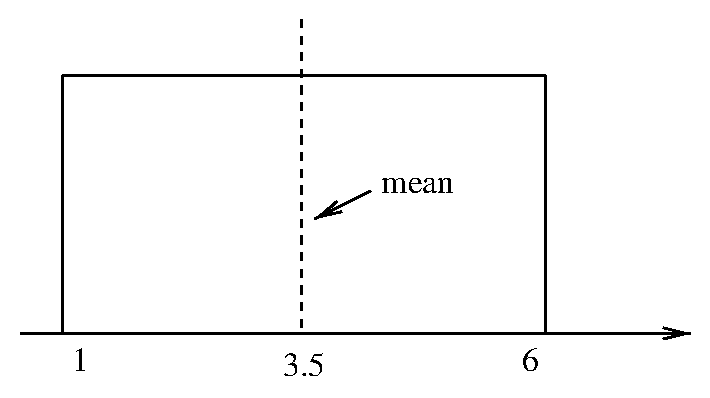
\includegraphics[height=2in]{figures/uniform}}
  \caption{This is a graph of the uniform distribution arising from
    rolling a fair die.  Outcomes within the range of the distribution
    are equally likely, regardless of distance from the mean.}
  \label{fig:uniform}
\end{figure}
\begin{figure}
  \centerline{\includegraphics[height=2in]{figures/binom2}}
  \caption{This is a rough graph of the binomial distribution given by
    the number of heads that come up when we flip 100 fair, mutually
    independent coins.  Outcomes close to the mean are much more
    likely than outcomes far from the mean.}
  \label{fig:binom2}
\end{figure}

On the other hand, we can define a random variable that always
deviates substantially from its expected value.  Suppose that we glue
100 coins together, so that with probability 1/2 all are heads and
with probability 1/2 all are tails.  The graph of the probability
distribution function for the number of heads is shown in
Figure~\ref{fig:nasty}.  While the expected value of this random
variable is 50, the actual value is always 0 or~100.
\begin{figure}
  \centerline{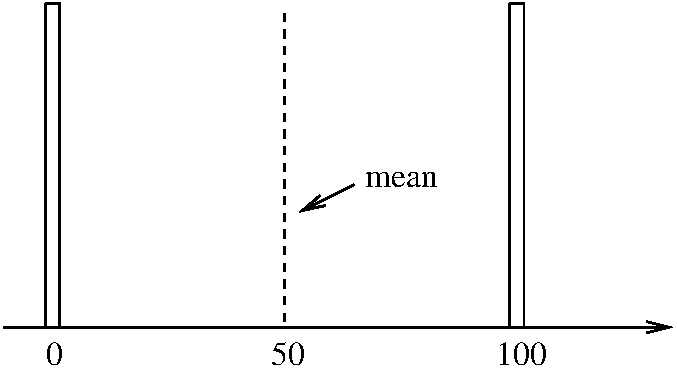
\includegraphics[height=2in]{figures/nasty}}
  \caption{This is the nasty distribution corresponding to the number
    of heads that come up when we flip 100 coins that are all glued
    together. The outcome always differs from the mean by at
    least~50.}
  \label{fig:nasty}
\end{figure}

Even in this last example, however, the random variable is twice the
mean with probability only $1/2$.  In fact, we will see that this is a
worst-case distribution with respect to deviation from the mean.


\subsection{Theorem Statement and Some Applications}
\fi

\begin{theorem}[Markov's Theorem]\label{markovthm}
  If R is a nonnegative random variable, then for all $x > 0$
  \begin{displaymath}
    \pr{R \geq x} \leq \frac{\expect{R}}{x}.
  \end{displaymath}
\end{theorem}

\iffalse

Before we prove Markov's Theorem, let's apply it to the three examples in
the preceding subsection.  First, let the random variable~$R$ be the
number that comes up when we roll a fair die.  By Markov's Theorem, the
probability of rolling a 6 is at most:
\[
\pr{R \geq 6} \leq \frac{\expect{R}}{6} = \frac{3.5}{6} = 0.583\dots
\]
This conclusion is true, but weak.  The actual probability of rolling
a 6 is $1/6 = 0.166\dots$.

This is typical of Markov's Theorem.  The theorem is easy to apply
because it requires so little information about a random variable,
only the expected value and nonnegativity.  But as a consequence,
Markov's Theorem often leads to weak conclusions like the one above.

Suppose that we flip 100 mutually independent, fair coins.  Markov's
Theorem says that the probability of throwing 75 or more heads is at
most:
\[
\pr{\text{heads} \geq 75} \leq \frac{\expect{\text{heads}}}{75} =
\frac{50}{75} = \frac{2}{3}.
\]
Markov's Theorem says that the probability of 75 or more heads is at
most $2/3$, but the actual probability is less than 1 in a
billion!

These two examples show that Markov's Theorem gives weak results for
well-behaved random variables; however, the theorem is actually tight
for some nasty examples.  Suppose we flip 100 fair coins and use
Markov's Theorem to compute the probability of getting all heads:
\[
\pr{\text{heads} \geq 100} \leq \frac{\expect{\text{heads}}}{100} =
\frac{50}{100} = \frac{1}{2}.
\]
If the coins are mutually independent, then the actual probability of
getting all heads is a miniscule 1 in $2^{100}$.  In this case, Markov's
Theorem looks very weak.  However, in applying Markov's Theorem, we made
no independence assumptions.  In fact, if all the coins are glued
together, then probability of throwing all heads is exactly $1/2$.
In this nasty case, Markov's Theorem is actually tight!

\subsection{Proof of Markov's Theorem}

Let $R$ be the weight of a person selected randomly and uniformly.
Suppose that an average person weighs 100 pounds; that is, $\expect{R} =
100$.  What is the probability that a random person weighs at least
200 pounds?

There is insufficient information for an exact answer.  However, we
can safely say that the probability that $R \geq 200$ is most
$1/2$.  If more than half of the people weigh 200 pounds or
more, then the average weight would exceed 100 pounds, even if
everyone else weighed zero!  Markov's Theorem gives the same result:
\begin{displaymath}
  \pr{R \geq 200} \leq \frac{\expect{R}}{200} = \frac{100}{200} = \frac{1}{2}.
\end{displaymath}

Reasoning similar to that above underlies the proof of Markov's
Theorem.  Since expectation is a weighted average of all the outcomes
of the random variable, that is, a sum over all the variables the random
variable can assume, we can give a lower bound on the expectation by
removing some of the terms from the sum defining the expectation; this
new sum can then be modified into an expression involving the
probability of an event in the tail $[R \geq x]$.
\fi

\begin{proof}%[Proof of Markov's Theorem]
We will show that $\expect{R} \geq x \pr{R \geq x}$.  Dividing
both sides by $x$ gives the desired result.

So let $I_x$ be the indicator variable for the event $[R \geq x]$, and
consider the random variable $x I_x$.  Note that
\[
R \geq x I_x,
\]
because at any sample point, $w$,
\begin{itemize}
\item if $R(\omega) \geq x$ then $R(\omega) \geq x = x\cdot 1 = x I_x(\omega)$, and
\item if $R(\omega) < x$ then $R(\omega) \geq 0 = x \cdot 0 = xI_x(\omega)$.
\end{itemize}
Therefore,
\begin{align*}
\expect{R} & \geq \expect{x I_x} & (\text{since } R \geq xI_x)\\
   & = x \expect{I_x} & \text{(linearity of $\expect{\cdot}$)}\\
   & = x \pr{I_x=1}  &  \text{($I_x$ is an indicator)}\\
   & = x \pr{R \geq x}.  &  (\text{def\ of $I_x$})
\end{align*}
\end{proof}

Markov's Theorem is often expressed in an alternative form, stated
below as an immediate corollary.
\begin{corollary}
If R is a nonnegative random variable, then for all $c \geq 1$
\begin{equation*}
\pr{R \geq c \cdot \expect{R}}  \leq  \frac{1}{c}.
\end{equation*}
\end{corollary}
\begin{proof}
In Markov's Theorem, set $x = c \cdot \expect{R}$.
\iffalse
This gives:
\[
\pr{R \geq c \cdot \expect{R}} \leq \frac{\expect{R}}{c \cdot \expect{R}} =
\frac{1}{c}.
\]
\fi
\end{proof}


\subsection{Applying Markov's Theorem}

Let's consider the Hat-Check problem again.  Now we ask what the
probability is that $x$ or more men get the right hat, this is, what the
value of $\pr{G \geq x}$ is.

We can compute an upper bound with Markov's Theorem.  Since we know
$\expect{G}=1$, Markov's Theorem implies
\[
\pr{G \geq x} \leq \frac{\expect{G}}{x} = \frac{1}{x}.
\]
For example, there is no better than a 20\% chance that 5 men get the
right hat, regardless of the number of people at the dinner party.

The Chinese Appetizer problem is similar to the Hat-Check problem.  In
this case, $n$ people are eating appetizers arranged on a circular,
rotating Chinese banquet tray.  Someone then spins the tray so that each
person receives a random appetizer.  What is the probability that everyone
gets the same appetizer as before?

There are $n$ equally likely orientations for the tray after it stops
spinning.  Everyone gets the right appetizer in just one of these $n$
orientations.  Therefore, the correct answer is $1/n$.

But what probability do we get from Markov's Theorem?  Let the random
variable, $R$, be the number of people that get the right appetizer.  
%We showed in previous notes that $\expect{R} = 1$.  
Then of course $\expect{R} = 1$ (right?), so
applying Markov's Theorem, we find:
\begin{displaymath}
  \pr{R \geq n} \leq \frac{\expect{R}}{n} = \frac{1}{n}\,.
\end{displaymath}
So for the Chinese appetizer problem, Markov's Theorem is tight!

On the other hand, Markov's Theorem gives the same $1/n$ bound for the
probability everyone gets their hat in the Hat-Check problem in the case
that all permutations are equally likely.  But the probability of this
event is $1/(n!)$.  So for this case, Markov's Theorem gives a probability
bound that is way off.

\subsubsection{Markov's Theorem for Bounded Variables}

Suppose we learn that the average \IQ\ among MIT students is 150 (which is
not true, by the way).  What can we say about the probability that an MIT
student has an \IQ\ of more than 200?  Markov's theorem immediately tells
us that no more than $150/200$ or $3/4$ of the students can have such a
high \IQ.  Here we simply applied Markov's Theorem to the random variable,
$R$, equal to the \IQ\ of a random MIT student to conclude:
\[
\pr{R > 200} \leq \frac{\expect{R}}{200}= \frac{150}{200} = \frac{3}{4}.
\]

But let's observe an additional fact (which may be true): no MIT student
has an \IQ\ less than 100.  This means that if we let $T \eqdef R-100$,
then $T$ is nonnegative and $\expect{T} = 50$, so we can apply Markov's
Theorem to $T$ and conclude:
\[
\pr{R > 200} = \pr{T > 100} \leq \frac{\expect{T}}{100}= \frac{50}{100} =
\frac{1}{2}.
\]
So only half, not 3/4, of the students can be as amazing as they think
they are.  A bit of a relief!

More generally, we can get better bounds applying Markov's Theorem to
$R-l$ instead of $R$ for any lower bound $l>0$ on $R$.

Similarly, if we have any upper bound, $u$, on a random variable, $S$,
then $u-S$ will be a nonnegative random variable, and applying Markov's
Theorem to $u-S$ will allow us to bound the probability that $S$ is much
\emph{less} than its expectation.

\iffalse

Suppose we know that $R \geq \ell$, then can we do better?
Let $T=R-\ell$.  Note that $T \geq 0$.  So, we can use Markov's
Theorem on $T$, to say that 
\begin{eqnarray*}
\pr{R  \geq x }   & = &   \pr{T \geq x -\ell} 
  \leq 
  \frac{\expect{T}}{x -\ell} 
  =   \frac{\expect{R - \ell}}{x - \ell}
  =   \frac{\expect{R} - \ell}{x - \ell} \\
  %& < &  \frac{\expect{R}}{x}
\end{eqnarray*}
%$\pr{R - \ell \geq x} = \pr{T \geq x} 
%\leq 
%\frac{\expect{T}}{x} 
%= \frac{\expect{R - \ell}}{x} =
%= \frac{\expect{R}{x} - \ell/x$
This gives a somewhat better bound on the probability that
$R$ goes crazy!  

\fi


\iffalse
\subsection{Why \emph{R} Must be Nonnegative}

Remember that Markov's Theorem applies only to nonnegative random
variables!  The following example shows that the theorem is false if this
restriction is removed.  Let $R$ be -10 with probability $1/2$ and 10 with
probability $1/2$.  Then we have:
\[
\expect{R} = -10 \cdot \frac{1}{2} + 10 \cdot \frac{1}{2} = 0
\]
Suppose that we now tried to compute $\pr{R \geq 5}$ using Markov's
Theorem:
\begin{displaymath}
  \pr{R \geq 5} \leq \frac{\expect{R}}{5} = \frac{0}{5} = 0.
\end{displaymath}
This is the wrong answer!  Obviously, $R$ is at least 5 with
probability $1/2$.  

On the other hand, we can still apply Markov's Theorem indirectly to
derive a bound on the probability that an arbitrary variable like $R$ is 5
more.  Namely, given any random variable, $R$ with expectation 0 and
values $\geq -10$, we can conclude that $\pr{R \geq 5} \le 2/3$.
\begin{proof}
Let $T \eqdef R+10$.  Now $T$ is a nonnegative random variable with
expectation $\expect{R + 10} = \expect{R}+10= 10$, so Markov's Theorem
applies and tells us that $\pr{T \geq 15} \le 10/15 = 2/3$.  But $T \geq
15$ iff $R \geq 5$, so $\pr{R \geq 5} \leq 2/3$, as claimed.
\end{proof}

\subsection{Deviation Below the Mean}

Markov's Theorem says that a random variable is unlikely to greatly exceed
the mean.  Correspondingly, there is a theorem that says a random variable
is unlikely to be much smaller than its mean.

\begin{theorem}
\label{th:below}
Let $l$ be a real number and let $R$ be a random variable such that $R
\leq l$.  For all $x < l$, we have:
\[
\pr{R \leq x} \leq \frac{l - \expect{R}}{l - x}.
\]
\end{theorem}

\begin{proof}
The event that $R \leq x$ is the same as the event that $l - R \geq l -
x$.  Therefore:
\begin{align}
\pr{R \leq x} &  = \pr{l - R \geq l - x}\notag\\
 & \leq \frac{\expect{l - R}}{l - x}. & \text{(by Markov' Theorem)}\label{LR}
\end{align}
Applying Markov's Theorem in line~(\ref{LR}) is permissible
since $l - R$ is a nonnegative random variable and $l - x > 0$.
\end{proof}

For example, suppose that the class average on the 6.042 midterm was
75/100.  What fraction of the class scored below 50?

There is not enough information here to answer the question exactly,
but Theorem~\ref{th:below} gives an upper bound.  Let $R$ be the score
of a random student.  Since 100 is the highest possible score, we
can set $L = 100$ to meet the condition in the theorem that $R \leq
L$.  Applying Theorem~\ref{th:below}, we find:
\begin{displaymath}
  \pr{R \leq 50} \leq \frac{100 - 75}{100 - 50} = \frac{1}{2}\,.
\end{displaymath}

That is, at most half of the class scored 50 or worse.  This makes
sense; if more than half of the class scored 50 or worse, then the
class average could not be 75, even if everyone else scored 100.
As with Markov's Theorem, Theorem~\ref{th:below} often gives weak
results.  In fact, based on the data given, the entire class could
have scored above 50.
\fi

\iffalse

\subsubsection{Using Markov To Analyze Non-Random Events [Optional]}
\begin{optional}

In the previous examples, we used a theorem about a random variable to
conclude facts about non-random data.  For example, we concluded that
if the average score on a test is 75, then at most $1/2$ the
class scored 50 or worse.  There is no randomness in this problem,
so how can we apply Theorem~\ref{th:below} to reach this conclusion?

The explanation is not difficult.  For any set of scores $S = \set{s_1,
s_2, \dots, s_n}$, we introduce a random variable, $R$, such that
\[
\pr{R = s_i} = \frac{\text{(\# of students with score $s_i$)}}{n}
\]
We then use Theorem~\ref{th:below} to conclude that $\pr{R \leq 50}
\leq 1/2$.  To see why this means (with certainty) that at most
$1/2$ of the students scored 50 or less, we observe that
\begin{eqnarray*}
\pr{R \leq 50}  & = & \sum_{s_i \leq 50} \pr{R = s_i} \\
  & = & \sum_{s_i \leq 50} \frac{\text{(\# of students with score $s_i$)}}{n} \\
  & = & \frac{1}{n} \text{(\# of students with score 50 or less)}.
\end{eqnarray*}
So, if $\pr{R \leq 50} \leq 1/2$, then the number of students
with score 50 or less is at most $n/2$.

\end{optional}
\fi

\subsection{Chebyshev's Theorem}

We have separate versions of Markov's Theorem for the probability of
deviation \emph{above} the mean and \emph{below} the mean, but often we
want bounds that apply to \emph{distance} from the mean in either
direction, that is, bounds on the probability that $\abs{R - \expect{R}}$
is large.

It is a bit messy to apply Markov's Theorem directly to this problem,
because it's generally not easy to compute $\expect{\ \abs{R -
\expect{R}}\ }$.  However, since $\abs{R}$ and hence $\abs{R}^k$ are
nonnegative variables for any $R$, Markov's inequality also applies to the
event $[\abs{R}^k \geq x^k]$.  But this event is equivalent to the event
$[\abs{R} \geq x]$, so we have:

\begin{lemma}\label{lem:Markov2}
For any random variable~$R$, any positive integer~$k$, and any $x > 0$,
\[
\pr{\abs{R} \geq x} \leq \frac{\expect{\abs{R}^k}}{x^k}.
\]
\end{lemma}

The special case of this Lemma for $k=2$ can be applied to bound the
random variable, $\abs{R - \expect{R}}$, that measures $R$'s deviation
from its mean.  Namely
\begin{equation}\label{chebE2}
\pr{\abs{R - \expect{R}} \geq x}
  = \pr{(R - \expect{R})^2 \geq x^2} \leq \frac{\expect{(R - \expect{R})^2}}{x^2},
\end{equation}
where the inequality~(\ref{chebE2}) follows by applying
Lemma~\ref{lem:Markov2} to the nonnegative random variable, $(R -
\expect{R})^2$.  Assuming that the quantity $\expect{(R - \expect{R})^2}$
above is finite, we can conclude that the probability that $R$ deviates
from its mean by more than~$x$ is $O(1/x^2)$.

\begin{definition}\label{defvar}
The \emph{variance}, $\variance{R}$, of a random variable, $R$, is:
\[
\variance{R} \eqdef \expect{(R - \expect{R})^2}.
\]
\end{definition}

So we can restate~(\ref{chebE2}) as
\begin{theorem}[Chebyshev]\label{chebthm}
Let $R$ be a random variable, and let $x$ be a positive real number.
Then
\[
\pr{\abs{R - \expect{R}} \geq x} \leq \frac{\variance{R}}{x^2}.
\]
\end{theorem}

The expression $\expect{(R - \expect{R})^2}$ for variance is a bit
cryptic; the best approach is to work through it from the inside out.  The
innermost expression, $R - \expect{R}$, is precisely the deviation of $R$
above its mean.  Squaring this, we obtain, $(R - \expect{R})^2$.  This is
a random variable that is near 0 when $R$ is close to the mean and is a
large positive number when $R$ deviates far above or below the mean.  So
if $R$ is always close to the mean, then the variance will be small.  If
$R$ is often far from the mean, then the variance will be large.

\subsubsection{Variance in Two Gambling Games}

The relevance of variance is apparent when we compare the following
two gambling games.

\textbf{Game A:} We win \$2 with probability $2/3$ and lose \$1 with probability
$1/3$.

\textbf{Game B:} We win \$1002 with probability $2/3$ and lose \$2001 with
probability $1/3$.

Which game is better financially?  We have the same probability, 2/3,
of winning each game, but that does not tell the whole story.  What about
the expected return for each game?  Let random variables $A$ and $B$ be
the payoffs for the two games.  For example, $A$ is 2 with probability
2/3 and -1 with probability 1/3.  We can compute the
expected payoff for each game as follows:
\begin{eqnarray*}
\expect{A} = 2 \cdot \frac{2}{3} + (-1) \cdot \frac{1}{3} = 1, \\
\expect{B} = 1002 \cdot \frac{2}{3} + (-2001) \cdot \frac{1}{3} = 1.
\end{eqnarray*}

The expected payoff is the same for both games, but they are obviously
very different!  This difference is not apparent in their expected value,
but is captured by variance.  We can compute the $\variance{A}$ by working
``from the inside out'' as follows:
\begin{eqnarray*}
A - \expect{A}
        & = &   \left\{
                \begin{array}{cl}
                        1 & \text{ with probability } \frac{2}{3} \\
                        -2 & \text{ with probability } \frac{1}{3}
                \end{array}
                \right. \\
(A - \expect{A})^2
        & = &   \left\{
                \begin{array}{cl}
                        1 & \text{ with probability } \frac{2}{3} \\
                        4 & \text{ with probability } \frac{1}{3}
                \end{array}
                \right. \\
\expect{(A - \expect{A})^2}
        & = &   1 \cdot \frac{2}{3} + 4 \cdot \frac{1}{3} \\
\variance{A} & = & 2.
\end{eqnarray*}

Similarly, we have for $\variance{B}$:
\begin{eqnarray*}
B - \expect{B}
        & = &   \left\{
                \begin{array}{cl}
                        1001 & \text{ with probability } \frac{2}{3} \\
                        -2002 & \text{ with probability } \frac{1}{3}
                \end{array}
                \right. \\
(B - \expect{B})^2
        & = &   \left\{
                \begin{array}{cl}
                        1,002,001 & \text{ with probability } \frac{2}{3} \\
                        4,008,004 & \text{ with probability } \frac{1}{3}
                \end{array}
                \right. \\
\expect{(B - \expect{B})^2}
        & = &   1,002,001 \cdot \frac{2}{3} + 4,008,004 \cdot \frac{1}{3} \\
\variance{B} & = & 2,004,002.
\end{eqnarray*}

The variance of Game A is 2 and the variance of Game B is more than
two million!  Intuitively, this means that the payoff in Game A is
usually close to the expected value of \$1, but the payoff in Game B
can deviate very far from this expected value.

High variance is often associated with high risk.  For example, in ten
rounds of Game A, we expect to make \$10, but could conceivably lose
\$10  instead.  On the other hand, in ten rounds of game B, we also
expect to make \$10, but could actually lose more than \$20,000!

\subsection{Standard Deviation}

Because of its definition in terms of the square of a random variable, the
variance of a random variable may be very far from a typical deviation
from the mean.  For example, in Game B above, the deviation from the mean
is 1001 in one outcome and -2002 in the other. But the variance is a
whopping 2,004,002.  From a dimensional analysis viewpoint, the ``units''
of variance are wrong: if the random variable is in dollars, then the
expectation is also in dollars, but the variance is in square dollars.
For this reason, people often describe random variables using standard
deviation instead of variance.

\begin{definition}
The \emph{standard deviation}, $\sigma_R$, of a random variable, $R$, is
the square root of the variance:
\[
\sigma_R \eqdef \sqrt{\variance{R}} = \sqrt{\expect{(R - \expect{R})^2}}.
\]      
\end{definition}

So the standard deviation is the square root of the mean of the square of
the deviation, or the ``root mean square'' for short.  It has the same
units---dollars in our example---as the original random variable and as
the mean.  Intuitively, it measures the ``expected (average) deviation
from the mean,'' since we can think of the square root on the outside as
canceling the square on the inside.

\begin{example}
The standard deviation of the payoff in Game B is:
\[
    \sigma_B  = \sqrt{\variance{B}} = \sqrt{2,004,002} \approx 1416.
\]

The random variable~$B$ actually deviates from the mean by either
positive 1001  or negative 2002; therefore, the standard
deviation of 1416 describes this situation reasonably well.
\end{example}

Intuitively, the standard deviation measures the ``width'' of the ``main
part'' of the distribution graph, as illustrated in
Figure~\ref{fig:stdev}.
\begin{figure}
  \centerline{\includegraphics[height=2in]{figures/stdev}}
  \caption{The standard deviation of a distribution indicates how wide the
    ``main part'' of it is.}
  \label{fig:stdev}
\end{figure}

There is a useful, simple reformulation of Chebyshev's Theorem in terms of
standard deviation.
\begin{corollary}
\label{cor:cheby}
Let $R$ be a random variable, and let $c$ be a positive real number.
\[
\pr{\abs{R - \expect{R}} \geq c \sigma_R} \leq \frac{1}{c^2}.
\]
\end{corollary}
Here we see explicitly how the ``likely'' values of $R$ are clustered in
an $O(\sigma_R)$-sized region around $\expect{R}$, confirming that the
standard deviation measures how spread out the distribution of $R$ is
around its mean.

\begin{proof}
  Substituting $x = c \sigma_R$ in Chebyshev's Theorem gives:
  \begin{displaymath}
    \pr{\card{R - \expect{R}} \geq c \sigma_R}
    \leq
    \frac{\variance{R}}{(c \sigma_R)^2}
    =  \frac{\sigma_R^2}{(c \sigma_R)^2}
    = \frac{1}{c^2}.
  \end{displaymath}
\iffalse
  The last equality holds because variance is the square of standard
  deviation: $\variance{R} = \sigma_R^2$.
\fi

\end{proof}

\subsubsection{The IQ\ Example}\label{IQsec}

Suppose that, in addition to the national average \IQ\ being 100, we also
know the standard deviation of \IQ's is 10.  How rare is an \IQ\ of 300 or
more?

Let the random variable, $R$, be the \IQ\ of a random person.  So we are
supposing that $\expect{R} = 100$, $\sigma_R = 10$, and $R$ is
nonnegative.  We want to compute $\pr{R \geq 300}$.

We have already seen that Markov's Theorem~\ref{markovthm} gives a coarse
bound, namely,
\[
  \pr{R \geq 300} \leq \frac{1}{3}.
\]
Now we apply Chebyshev's Theorem to the same problem:
\[
\pr{R \geq 300} = \pr{\abs{R - 100} \geq 200} \leq
\frac{\variance{R}}{200^2} = \frac{10^2}{200^2} = \frac{1}{400}.
\]
The purpose of the first step is to express the desired probability in the
form required by Chebyshev's Theorem; the equality holds because $R$ is
nonnegative.  Chebyshev's Theorem then yields the inequality.

So Chebyshev's Theorem implies that at most one person in four hundred has
an \IQ\ of 300 or more.  We have gotten a much tighter bound using the
additional information, namely the variance of $R$, than we could get
knowing only the expectation.

\subsection{Properties of Variance}

The definition of variance of $R$ as $\expect{(R - \expect{R})^2}$ may
seem rather arbitrary.
\iffalse
The variance is the average \emph{of the square} of the deviation from the
mean.  For this reason, variance is sometimes called the ``mean squared
deviation.''  But why bother squaring?  Why not simply compute the average
deviation from the mean?  That is, why not define variance to be
$\expect{R - \expect{R}}$?

The problem with this definition is that the positive and negative
deviations from the mean exactly cancel.  By linearity of expectation,
we have:
\[
  \expect{R - \expect{R}} = \expect{R} - \expect{\expect{R}}.
\]
Since $\expect{R}$ is a constant, its expected value is itself. Therefore
\[
\expect{R - \expect{R}} = \expect{R} - \expect{R} = 0.
\]
By this definition, every random variable has zero variance.  That is not
useful!  Because of the square in the conventional definition, both
positive and negative deviations from the mean increase the variance;
positive and negative deviations do not cancel.

Of course, we could also prevent positive and negative deviations from
canceling by taking an absolute value.\fi A direct measure of average
deviation would be $\expect{\ \abs{R - \expect{R}}\ }$.  But variance has
some valuable mathematical properties which the direct measure does not,
as we explain below.

\iffalse
For example, for independent random variables, the variance of a sum
is the sum of the variances; that is, $\variance{R_1 + R_2} =
\variance{R_1} + \variance{R_2}$.  We will prove this fact below.
\fi

\subsubsection{A Formula for Variance}

Applying linearity of expectation to the formula for variance yields a convenient
alternative formula.
\begin{theorem}\label{alt:var}
\[
\variance{R} = \expect{R^2} - \expectsq{R},
\]
for any random variable, $R$.
\end{theorem}
Here we use the notation $\expectsq{R}$ as shorthand for $(\expect{R})^2$.

\iffalse
Remember that $\expect{R^2}$ is generally not equal to $\expectsq{R}$.  We
know the expected value of a product is the product of the expected values
for independent variables, but not in general.  And $R$ is not independent
of itself unless it is constant.\fi

\begin{proof}
Let $\mu = \expect{R}$.  Then
\begin{align*}
\variance{R} & =   \expect{(R - \expect{R})^2}
               & \text{(Def~\ref{defvar} of variance)}\\
        & = \expect{(R - \mu)^2} & \text{(def of $\mu$)}\\
        & = \expect{R^2 - 2  \mu R + \mu^2} \\
        & = \expect{R^2} - 2 \mu \expect{R} + \mu^2 
                & \text{(linearity of expectation)}\\
        & = \expect{R^2} - 2 \mu^2 + \mu^2
              &  \text{(def of $\mu$)}\\
        & = \expect{R^2} - \mu^2\\
        & = \expect{R^2} - \expectsq{R}.
                  &  \text{(def of $\mu$)}
\end{align*}
\end{proof}

For example, if $B$ is a Bernoulli variable where $p\eqdef \pr{B=1}$, then
\begin{equation}\label{bv}
\variance{B} = p-p^2 = p(1-p).
\end{equation}
\begin{proof}
Since $B$ only takes values 0 and 1, we have $\expect{B}=p\cdot 1 + (1-p)
\cdot 0 = p$.  Since $B = B^2$, we also have $\expect{B^2} = p$,
so~\eqref{bv} follows immediately from Theorem~\ref{alt:var}.
\end{proof}

\iffalse
\begin{optional}

Theorem~\ref{alt:var} gives a convenient way to compute the variance of a
random variable: find the expected value of the square and subtract the
square of the expected value.  For example, we can compute the variance of
the outcome of a fair die as follows:
\begin{gather*}
  \expect{R^2} = \frac{1}{6} (1^2 + 2^2 + 3^2 + 4^2 + 5^2 + 6^2) = \frac{91}{6}, \\
  \expectsq{R} = \left(3 \frac{1}{2}\right)^2 = \frac{49}{4}, \\
  \variance{R}  = \expect{R^2} - \expectsq{R}
  = \frac{91}{6} - \frac{49}{4} = \frac{35}{12}.
\end{gather*}

This result is particularly useful when we want to estimate the variance
of a random variable from a sequence $x_1,x_2,\dots,x_n$, of sample values
of the variable.

\begin{definition}
For any sequence of real numbers $x_1,x_2,\dots,x_n$, define the
\emph{sample mean}, $\mu_n$, and the \emph{sample variance}, $v_n$, of the
sequence to be:
\begin{eqnarray*}
\mu_n  & \eqdef & \frac{\sum_{i=1}^n x_i}{n},\\
v_n  & \eqdef & \frac{\sum_{i=1}^n (x_i - \mu_n)^2}{n}.
\end{eqnarray*}
\end{definition}
Notice that if we define a random variable, $R$, which is equally likely
to take each of the values in the sequence, that is $\pr{R = x_i} = 1/n$
for $i = 1,\dots,n$, then $\mu_n = \expect{R}$ and $v_n = \variance{R}$.
So Theorem~\ref{alt:var} applies to $R$ and lets us conclude that
\begin{equation}\label{vn:alt}
v_n = \frac{\sum_{i=1}^n x_i^2}{n} - \left(\frac{\sum_{i=1}^n x_i}{n}\right)^2.
\end{equation}
This leads to a simple procedure for computing the sample mean and
variance while reading the sequence $x_1,\dots,x_n$ from left to right.
Namely, maintain a sum of all numbers seen and also maintain a sum of the
squares of all numbers seen.  That is, we store two values, starting with
the values $x_1$ and $x_1^2$.  Then, as we get to the next number, $x_i$,
we add it to the first sum and add its square, $x_{i}^2$, to the second
sum.  After a single pass through the sequence $x_1,\dots,x_n$, we wind up
with the values of the two sums $\sum_{i=1}^n x_i$ and $\sum_{i=1}^n
x_i^2$.  Then we just plug these two values into~(\ref{vn:alt}) to find
the sample variance.

\end{optional}
\fi

\iffalse

\subsubsection{Expectation Squared [Optional]}

\begin{optional}

The alternate definition of variance given in Theorem~\ref{alt:var} has
a cute implication:
\begin{corollary}
If $R$ is a random variable, then $\expect{R^2} \geq \expectsq{R}$.
\end{corollary}
\begin{proof}
We first defined $\variance{R}$ as an average of a squared expression, so
$\variance{R}$ is nonnegative.  Then we proved that $\variance{R} =
\expect{R^2} - \expectsq{R}$.  This implies that $\expect{R^2} -
\expectsq{R}$ is nonnegative.  Therefore, $\expect{R^2} \geq
\expectsq{R}$.
\end{proof}

In words, the expectation of a square is at least the square of the
expectation. The two are equal exactly when the variance is zero:
\begin{displaymath}
\expect{R^2} = \expectsq{R} \text{  iff  } \expect{R^2} - \expectsq{R} = 0
\text{  iff  } \variance{R} = 0.
\end{displaymath}

\end{optional}
\fi

\iffalse

\subsubsection{Zero Variance}

When does a random variable, $R$, have zero variance?\dots when the random
variable \emph{never} deviates from the mean!
\begin{lemma}\label{zvar}
The variance of a random variable, $R$, is zero if and only if $\pr{R =
\expect{R}} = 1$.
\end{lemma}

So saying that $\variance{R}=0$ is almost the same as saying that $R$ is
constant.  Namely, it takes the constant value equal to its expectation on
all sample points with nonzero probability.  (It can take on any finite
values on sample points with zero probability without affecting the
variance.)

\begin{proof}
By the definition of variance,
\[
\variance{R} = 0\qiff \expect{(R - \expect{R})^2} = 0.
\]
The inner expression on the right, $(R - \expect{R})^2$, is always
nonnegative because of the square.  As a result, $\expect{(R -
\expect{R})^2} = 0$ if and only if $\pr{(R - \expect{R})^2 \neq 0}$ is
zero, which is the same as saying that $\pr{(R - \expect{R})^2 = 0}$ is
one.  That is,
\[
\variance{R} = 0 \qiff \pr{(R - \expect{R})^2 = 0} = 1.
\]
But the $(R - \expect{R})^2 = 0$ and $R = \expect{R}$ are different
descriptions of the same event.  Therefore,
\[
\variance{R} = 0 \qiff \pr{R = \expect{R}} =1.
\]
\end{proof}
\fi

\subsubsection{Dealing with Constants}

It helps to know how to calculate the variance of $aR+b$:

\begin{theorem}\label{var.const}
Let $R$ be a random variable, and $a$ a constant. Then
\begin{equation}\label{a2R}
\variance{a R} = a^2 \variance{R}.
\end{equation}
\end{theorem}

\begin{proof}
Beginning with the definition of variance and repeatedly applying
linearity of expectation, we have:
\begin{align*}
\variance{aR}
    & \eqdef \expect{(aR-\expect{aR})^2}\\
    & = \expect{(aR)^2 -2aR\expect{aR} + \expectsq{aR}}\\
    & = \expect{(aR)^2} -\expect{2aR\expect{aR}} + \expectsq{aR}\\
    & = a^2\expect{R^2} -2\expect{aR}\expect{aR} + \expectsq{aR}\\
    & = a^2\expect{R^2} -a^2\expectsq{R}\\
    & = a^2\paren{\expect{R^2} - \expectsq{R}}\\
    & = a^2\variance{R} & \text{(by Theorem~\ref{alt:var})}
\end{align*}
\end{proof}

It's even simpler to prove that adding a constant does not change the
variance, as the reader can verify:
\begin{theorem}\label{var+const}
Let $R$ be a random variable, and $b$ a constant. Then
\begin{equation}\label{R+b}
\variance{R+b} = \variance{R}.
\end{equation}
\end{theorem}

\insolutions{
\begin{proof}
\begin{align*}
\variance{R+b} & \eqdef \expect{((R+b) - \expect{R+b})^2}\\
               & =  \expect{((R+b) - (\expect{R}+ b))^2}\\
               & =  \expect{(R - \expect{R})^2}\\
               & = \variance{R}.
\end{align*}
\end{proof}
}

Recalling that the standard deviation is the square root of variance, we
immediately get:
\begin{corollary}
The standard deviation of $a R + b$ equals $\abs{a}$ times the standard
deviation of $R$:
\[
\sigma_{aR+b} = \abs{a}\sigma_{R}.
\]
\end{corollary}


\subsubsection{Variance of a Sum}

In general, the variance of a sum is not equal to the sum of the variances,
but variances do add for \emph{independent} variables.  In fact,
\emph{mutual} independence is not necessary: \emph{pairwise} independence
will do.  This is useful to know because there are some important
situations involving variables that are pairwise independent but not
mutually independent.

\iffalse
\begin{theorem}\label{indvar}
If $R_1$ and $R_2$ are independent random variables, then
\begin{equation}\label{vR+R}}
\variance{R_1 + R_2} = \variance{R_1} + \variance{R_2}.
\end{equation}
\end{theorem}

\begin{proof}
We may assume that $\expect{R_i} = 0$ for $i=1,2$, since we could always
replace $R_i$ by $R_i-\expect{R_i}$ in equation~\eqref{vR+R}.  This
substitution preserves the independence of the variables, and by
Theorem~\ref{var+const}, does not change the variances.

Now by Theorem~\ref{alt:var}, $\variance{R_i} = \expect{R_i^2}$ and
$\variance{R_1+R_2} = \expect{(R_1+R_2)^2}$, so we need only prove
\begin{equation}\label{E2R+R}
\expect{(R_1+R_2)^2} = \expect{R_1^2} + \expect{R_2^2}.
\end{equation}
But~\eqref{ follows from linearity of expectation and the fact that
\begin{equation}\label{rrind}}
\expect{R_1R_2} = \expect{R_1}\expect{R_2}
\end{equation}
since $R_1$ and $R_2$ are independent:
\begin{align*}
\expect{(R_1+R_2)^2}
   & = \expect{R_1^2+2R_1R_2 +R_2^2}\\
   & = \expect{R_1^2}+2\expect{R_1R_2} +\expect{R_2^2}\\
   & = \expect{R_1^2}+2\expect{R_1}\expect{R_2} +\expect{R_2^2}
             & \text{(by~\eqref{rrind})}\\
   & = \expect{R_1^2}+2\cdot 0 \cdot 0 +\expect{R_2^2}\\
   & =  \expect{R_1^2} + \expect{R_2^2}
\end{align*}
\fi

\iffalse
We will transform the left side into the right side.  We begin by
applying the alternate definition of variance.
\[
\variance{R_1 + R_2} = \expect{(R_1 + R_2)^2} - \expectsq{R_1 + R_2}.
\]

We will work on the first term and then the second term separately.
For the first term, note\begin{eqnarray*}
\expect{(R_1+R_2)^2}
& = &   \expect{R_1^2 + 2 R_1 R_2 + R_2^2} \\
& = &   \expect{R_1^2} + \expect{2 R_1 R_2} + \expect{R_2^2} \\
& = &   \expect{R_1^2} + 2 \expect{R_1} \expect{R_2} + \expect{R_2^2}.
\end{eqnarray*}
First, we multiply out the squared expression.  The second step uses
linearity of expectation.  In the last step, we break the
expectation of the product $R_1 R_2$ into a product of expectations;
this is where we use the fact that $R_1$ and $R_2$ are independent.
Now we work on the second term.
\begin{eqnarray*}
\expectsq{R_1+R_2} & = & (\expect{R_1} + \expect{R_2})^2 \\
& = & \expectsq{R_1} + 2 \expect{R_1} \expect{R_2} + \expectsq{R_2}.
\end{eqnarray*}
The first step uses linearity of expectation, and in the second step
we multiply out the squared expression.  Now we subtract the
(expanded) second term from the first. Cancelling and rearranging
terms, we find that
\begin{eqnarray*}
\variance{R_1 + R_2} & = &   (\expect{R_1^2} - \expectsq{R_1}) +
(\expect{R_2^2}) - \expectsq{R_2}) \\
& = &   \variance{R_1} + \variance{R_2}.
\end{eqnarray*}

\end{proof}

An independence condition is necessary.  If we ignored independence, then
we would conclude that $\variance{R + R} = \variance{R} + \variance{R}$.
However, by Theorem~\ref{var.const}, the left side is equal to $4
\variance{R}$, whereas the right side is $2 \variance{R}$.  This implies
that $\variance{R}=0$, which, by Lemma~\ref{zvar}, essentially only holds
if $R$ is constant.
\fi


\begin{theorem}\label{th:varsum}[Pairwise Independent Additivity of Variance]
If $R_1, R_2, \dots, R_n$ are \emph{pairwise} independent random
variables, then
\begin{equation}\label{vsum}
\variance{R_1 + R_2 + \cdots + R_n} = \variance{R_1} + \variance{R_2} +
  \cdots + \variance{R_n}.
\end{equation}
\end{theorem}

\begin{proof}
We may assume that $\expect{R_i} = 0$ for $i=1,\dots,n$, since we could
always replace $R_i$ by $\paren{R_i-\expect{R_i}}$ in
equation~\eqref{vsum}.  This substitution preserves the independence of
the variables, and by Theorem~\ref{var+const}, does not change the
variances.

Now by Theorem~\ref{alt:var}, $\variance{R_i} = \expect{R_i^2}$ and
$\variance{R_1+R_2+\cdots+R_n} = \expect{(R_1+R_2+\cdots+R_n)^2}$, so we
need only prove
\begin{equation}\label{E2R+R}
\expect{(R_1+R_2+\cdots+R_n)^2} = \expect{R_1^2} + \expect{R_2^2} + \cdots
+ \expect{R_n^2}
\end{equation}
But~\eqref{E2R+R} follows from linearity of expectation and the fact that
\begin{equation}\label{rrind}
\expect{R_iR_j} = \expect{R_i}\expect{R_j} = 0 \cdot 0 = 0
\end{equation}
for $i \neq j$, since $R_i$ and $R_j$ are independent.
\begin{align*}
\expect{(R_1+R_2+\cdots+R_n)^2}
   & = \expect{\sum_{1\leq i,j \leq n} R_iR_j}\\
   & = \sum_{1\leq i,j \leq n} \expect{R_iR_j}\\
   & = \sum_{1 \leq i \leq n} \expect{R_i^2}
             + \sum_{1 \leq i \neq j \leq n} \expect{R_iR_j}\\
   & = \sum_{1 \leq i \leq n} \expect{R_i^2}
            + \sum_{1 \leq i \neq j \leq n} 0 
             & \text{(by~\eqref{rrind})}\\
   & =  \expect{R_1^2} + \expect{R_2^2} + \cdots + \expect{R_n^2}.
\end{align*}

\iffalse
By linearity of expectation, we have
\begin{align}
\expect{\biggl(\sum_{i=1}^n R_i\biggr)^2} &
    = \expect{\sum_{i=1}^n \sum_{j=1}^n R_i R_j} \notag\\
   &  = \sum_{i=1}^n \sum_{j=1}^n \expect{R_i R_j} & \text{(linearity)}\notag\\
   & = \sum_{1\le i \neq j \le n} \expect{R_i}\expect{R_j} + \sum_{i=1}^n
     \expect{R_i^2}.
       & \text{(pairwise independence)} \label{ER2}
\end{align}
In~(\ref{ER2}), we use the fact that the expectation
of the product of two independent variables is the product of their
expectations.

Also,
\begin{align}
\expectsq{\sum_{i=1}^n R_i} & = \biggl(\expect{\sum_{i=1}^n R_i}\biggr)^2 \notag\\
  &  = \biggl(\sum_{i=1}^n \expect{R_i}\biggr)^2 &\text{(linearity)} \notag\\
  &  = \sum_{i=1}^n \sum_{j=1}^n \expect{R_i} \expect{R_j}\notag\\
  & = \sum_{1\le i \neq j \le n} \expect{R_i}\expect{R_j} + \sum_{i=1}^n
     \expectsq{R_i}.\label{E2R}
\end{align}
So,
\begin{align*}
\variance{\biggl(\sum_{i=1}^n R_i\biggr)}
   & =  \expect{\biggl(\sum_{i=1}^n R_i\biggr)^2} -
\expectsq{\sum_{i=1}^n R_i}  & \text{(Theorem~\ref{alt:var})}\\
   &  = \sum_{1\le i \neq j \le n} \expect{R_i} \expect{R_j}
        + \sum_{i=1}^n \expect{R_i^2} - \\
   & \quad \paren{\sum_{1\le i \neq j \le n} \expect{R_i}\expect{R_j}
        + \sum_{i=1}^n \expectsq{R_i}}
      & \text{(by~(\ref{ER2}) and~(\ref{E2R}))}\\
   & = \sum_{i=1}^n \expect{R_i^2} - \sum_{i=1}^n \expectsq{R_i}\\
   & = \sum_{i=1}^n (\expect{R_i^2} - \expectsq{R_i})
             & \text{(reordering the sums)}\\
   & = \sum_{i=1}^n \variance{R_i}. & \text{(Theorem~\ref{th:alt})}
\end{align*}
\fi

\end{proof}

Now we have a simple way of computing the variance of a variable, $J$,
that has an $(n,p)$-binomial distribution.  We know that $J =
\sum_{k=1}^n I_k$ where the $I_k$ are mutually independent 0-1-valued
variables with $\pr{I_k=1}=p$.  The variance of each $I_k$ is $p(1-p)$
by~\eqref{bv}, so by linearity of variance, we have
\begin{lemma*}[Variance of the Binomial Distribution]
If $J$ has the $(n,p)$-binomial distribution, then
\begin{equation}\label{p1p}
\variance{J} = n \variance{I_k} = np(1-p).
\end{equation}
\end{lemma*}

%\subsection{Applying Chebyshev's Theorem}

\subsection{Estimation by Random Sampling}

\subsubsection{Polling again}

In Notes 12, we used bounds on the binomial distribution to determine
confidence levels for a poll of voter preferences of Franken vs.\ Coleman.
Now that we know the variance of the binomial distribution, we can use
Chebyshev's Theorem as an alternative approach to calculate poll size.

The setup is the same as in Notes 12: we will poll $n$ randomly chosen
voters and let $S_n$ be the total number in our sample who preferred
Franken.  We use $S_n/n$ as our estimate of the actual fraction, $p$, of
all voters who prefer Franken.  We want to choose $n$ so that our estimate
will be within $0.04$ of $p$ at least 95\% of the time.

Now $S_n$ is binomially distributed, so from~\eqref{p1p} we have
\[
\variance{S_n}  = n(p(1-p)) \leq n \cdot \frac{1}{4} = \frac{n}{4}\label{n4}
\]
The bound of 1/4 follows from the fact that $p(1-p)$ is maximized when $p
= 1-p$, that is, when $p=1/2$ (check this yourself!).

Next, we bound the variance of $S_n/n$:
\begin{align}
\variance{\frac{S_n}{n}}
       & = \paren{\frac{1}{n}}^2 \variance{S_n}
                     & \text{(by~\eqref{a2R})}\notag\\
       & \leq \paren{\frac{1}{n}}^2 \frac{n}{4} & \text{(by~\eqref{n4})}\notag\\
       & = \frac{1}{4n}\label{1/4n}
\end{align}
Now from Chebyshev and~\eqref{1/4n} we have:
\begin{equation}\label{CK}
\pr{\abs{\frac{S_n}{n} - p} \geq 0.04}
    \leq \frac{\variance{S_n/n}}{(0.04)^2}
       = \frac{1}{4n(0.04)^2} = \frac{156.25}{n}
\end{equation}

To make our our estimate with  95\% confidence, we want the righthand
side of~\eqref{CK} to be at most 1/20.  So we choose $n$ so that
\[
\frac{156.25}{n} \leq \frac{1}{20},
\]
that is,
\[
n \geq 3,125.
\]

You may remember that in Notes 12 we calculated that it was actually
sufficient to poll only 664 voters ---many fewer than the 3,125 voters we
derived using Chebyshev's Theorem.  So the bound from Chebyshev's Theorem
is not nearly as good as the bound we got earlier.  This should not be
surprising.  In applying the Chebyshev Theorem, we used only a bound on
the variance of $S_n$.  In Notes 12, on the other hand, we used the fact
that the random variable $S_n$ was binomial (with known parameter, $n$,
and unknown parameter, $p$).  It makes sense that more detailed
information about a distribution leads to better bounds.  But even though
the bound was not as good, this example nicely illustrates an approach to
estimation using Chebyshev's Theorem that is more widely applicable than
binomial estimations.

\subsubsection{Matching Birthdays}

There are important cases where the relevant distributions are not binomial
because the mutual independence properties of the voter preference example
do not hold.  In these cases, estimation methods based on the Chebyshev
bound may be the best approach.  Birthday Matching is an example: suppose
we have 100 students in a classroom.  What is the probability that there is
a pair of students with the same birthday?  The answer to this question
surprises most people: it turns out it is virtually certain, namely
0.999999.  Before we explain this answer, we better explain our probability
model.

\begin{itemize}

\item Let $n$ be the number of students in the class.

\item Let $d$ be the number of days in the year.

\item Let $D$ be the number of pairs of students with the same birthday.

\end{itemize}

Ignoring leap years, $d= 365$, but we'll really study the case when $d$ is
an arbitrary positive integer.  Our first assumption is that the
probability that a randomly chosen student has a given birthday is $1/d$.
This assumption is not really true, since more babies are born at certain
times of year.  However, our analysis of this problem applies to many
situations in Computer Science that are unaffected by leap days, snow days
or Spring fever, so we won't dwell on those complications.  We'll also
assume that the $n$ students in the class are chosen randomly from the
population of students, with each student equally likely to be chosen, and
choices made independently.

A sensible sample space to model this experiment consists of all ways of
assigning birthdays to the students in the class.  There are $d^n$ such
assignments, since the first person can have $d$ different birthdays, the
second person can have $d$ different birthdays, and so forth.
Furthermore, every such assignment is equally probable by our assumption
that birthdays are equally likely and independent of each other.

Now the event that some two students have the same birthday can be
expressed as $[D>0]$.  It turns out to be be easier to calculate the
complement event $[D=0]$ that everyone has a distinct birthday, which is
good enough since $\pr{D>0} = 1 - \pr{D=0}$.  At this point we have all the
assumptions needed to calculate this probability explicitly, but instead we
will ask a somewhat different question: \emph{how many} matching pairs of
birthdays should we expect, and what is the \emph{probability of getting
close} to this expected number?

Now it will be easy to calculate the expected number of pairs of students
with matching birthdays.  Then we can take the same approach as we did in
estimating voter preferences to get an estimate of the probability of
getting a number of pairs close to the expected number.

But notice that, unlike the situation with voter preferences, having
matching birthdays for different pairs of students are not mutually
independent events.  For example, knowing that Alice and Bob have matching
birthdays, and also that Ted and Alice have matching birthdays obviously
implies that Bob and Ted have matching birthdays.  On the other hand,
knowing that Alice and Bob have matching birthdays tells us nothing about
whether Alice and Carol have matching birthdays, namely, these two events
really are independent.  So even though the events that various pairs of
students have matching birthdays are not mutually independent, indeed not
even three-way independent, they are \emph{pairwise} independent.

%We already observed this
%phenomenon for the case of matching pairs among three coins in
%\href{http://theory.lcs.mit.edu/classes/6.042/fall03/handouts/ln10.pdf}
%{Notes 10}, \S12.7.  

This will allow us to apply the same reasoning to Birthday Matching as we
did for voter preference.  Namely, let $B_1,B_2,\dots,B_n$ be the birthdays
of $n$ independently chosen people, and let $E_{i,j}$ be the indicator
variable for the event that the $i$th and $j$th people chosen have the same
birthdays, that is, the event $[B_i = B_j]$.  According to our probabillity
model, the $B_i$'s are mutually independent variables, and hence the
$E_{i,j}$'s are \emph{pairwise} independent variables, which is all we will
need.  Also, the expectations of $E_{i,j}$ for $i \neq j$ equals the
probability that $B_i = B_j$, namely, $1/d$.

Now, $D$, the number of matching pairs of birthdays among the $n$
choices is simply the sum of the $E_{i,j}$'s:
\begin{equation}\label{Vn}
D \eqdef \sum_{1\le i < j \le n} E_{i,j}.
\end{equation}
So by linearity of expectation
\[
\expect{D} = \expect{\sum_{1\le i < j \le n} E_{i,j}} = 
               \sum_{1\le i < j \le n} \expect{E_{i,j}} =
               \binom{n}{2}\cdot \frac{1}{d}.
\]
Also, by Theorem~\ref{th:varsum}, the variances of pairwise independent
variables are additive, so
\[
\variance{D} = \variance{\sum_{1\le i < j \le n} E_{i,j}} = 
               \sum_{1\le i < j \le n} \variance{E_{i,j}} =
               \binom{n}{2} \cdot \frac{1}{d}\paren{1-\frac{1}{d}}.
\]

In particular, for a class of $n= 100$ students with $d=365$ possible
birthdays, we have $\expect{D} \approx 14$ and $\variance{D} < 14 (1-
1/365) < 14$.  So by Chebyshev's Theorem
\[
\pr{\abs{D - 14} \geq x} < \frac{14}{x^2}.
\]

Letting $x=6$, we conclude that there is a better than 50\% chance that in
a class of 100 students, the number of pairs of students with the same
birthday will be between 8 and 20.  

%In fact, there turned out to be
%\emph{exactly} the 16 matches expected in the class this term!

\iffalse
Add another calculation, say for a 6.001 class of 400, or for uniform
selection of numbers from 1 to 1,000,000.
\fi

\hyperdef{pairwise}{independent}{\subsection{Pairwise Independent Sampling}}

The reasoning we used above to analyze voter polling and matching
birthdays is very similar.  We summarize it in slightly more general form
with a basic result we call the Pairwise Independent Sampling Theorem.  In
particular, we do not need to restrict ourselves to sums of zero-one
valued variables, or to variables with the same distribution.  For
simplicity, we state the Theorem for pairwise independent variables with
possibly different distributions but with the same mean and variance.

\begin{theorem*}[Pairwise Independent Sampling]
Let $G_1, \dots, G_n$ be pairwise independent variables with the same
mean, $\mu$, and deviation, $\sigma$ .  Define
\begin{equation}\label{ln14.Sn}
S_n \eqdef \sum_{i=1}^n G_i.
\end{equation}
Then
\[
\pr{\abs{\frac{S_n}{n} - \mu} \geq x}
    \leq \frac{1}{n} \paren{\frac{\sigma}{x}}^2.
\]
\end{theorem*}

\begin{proof}
We observe first that the expectation of $S_n/n$ is $\mu$:
\begin{align*}
\expect{\frac{S_n}{n}} & = \expect{\frac{\sum_{i=1}^n G_i}{n}}
         & \text{(def of $S_n$)}\\
 & = \frac{\sum_{i=1}^n \expect{G_i}}{n} 
     & \text{(linearity of expectation)}\\
 & = \frac{\sum_{i=1}^n \mu}{n}\\
 & = \frac{n\mu}{n} = \mu.
\end{align*}

The second important property of $S_n/n$ is that its variance is the
variance of $G_i$ divided by $n$:
\begin{align}
\variance{\frac{S_n}{n}} & =  \paren{\frac{1}{n}}^2 \variance{S_n}
          & \mbox{(by~\eqref{a2R})}\notag\\
 & =  \frac{1}{n^2} \variance{\sum_{i=1}^n G_i} 
          & \text{(def of $S_n$)}\notag\\
 & =  \frac{1}{n^2} \sum_{i=1}^n \variance{G_i}
        & \text{(pairwise independent additivity)}\notag\\
 & =  \frac{1}{n^2}\cdot n\sigma^2 =  \frac{\sigma^2}{n}.\label{Snu}
\end{align}

This is enough to apply Chebyshev's Bound and conclude:
\begin{align*}
\pr{\abs{\frac{S_n}{n} - \mu} \geq x} & \leq \frac{\variance{S_n/n}}{x^2}.
       & \text{(Chebyshev's bound)}\\
    & = \frac{\sigma^2/n}{x^2} & \text{(by~(\ref{Snu}))}\\
    & = \frac{1}{n} \paren{\frac{\sigma}{x}}^2.
\end{align*}

\end{proof}

The Pairwise Independent Sampling Theorem provides a precise general
statement about how the average of independent samples of a random
variable approaches the mean.  In particular, it proves what is known as
the Law\footnote{This is the \emph{Weak} Law of Large Numbers.  As you
might suppose, there is also a Strong Law, but it's outside the scope of
6.042.} of Large Numbers: by choosing a large enough sample size, $n$, we
can get arbitrarily accurate estimates of the mean with confidence
arbitrarily close to 100\%.

%% Variance Problems %%%%%%%%%%%%%%%%%%%%%%%%%%%%%%%%%%%%%%%%%%%%%%%%%%%%%%%%%%
%\startclassproblems
%\pinput{CP_}


%% Conclusion %%%%%%%%%%%%%%%%%%%%%%%%%%%%%%%%%%%%%%%%%%%%%%%%%%%%%%%%%%%%%%%%%
\TBA{Conclusion...}

\endinput
